\documentclass{article}
% Package to manage page layout
\usepackage[margin=1.5cm, includefoot, footskip=30pt]{geometry}

\setlength\parindent{0pt}
\setlength{\parskip}{1em}

%%%%%%%PACKAGES HERE%%%%%%%
\usepackage{amsmath}
\usepackage{hyperref}
\usepackage{standalone}
\usepackage{subcaption}
\usepackage{tikz}
\usepackage{booktabs}
\usepackage{minted}
\usepackage{multicol}
\usetikzlibrary{er,positioning, calc}

\definecolor{background}{RGB}{5, 66, 81}
\usemintedstyle{tango}


\newcommand{\totalarticles}{\input{assets/total_articles.txt}}
\newcommand{\uniquetitles}{\input{assets/unique_titles.txt}}
\newcommand{\numberofduplicates}{\input{assets/number_of_duplicates.txt}}
\newcommand{\manual}{\input{assets/prov_manual.txt}}
\newcommand{\authors}{\input{assets/authors.txt}}
%%%%%%%%%%%%%%%%%%%%%%%%%%%
\title{Literature review paper for the iterated prisoner's dilemma.}
\author{Nikoleta E. Glynatsi}
\date{2016}

\begin{document}

\maketitle

\section{Introduction}\label{section:introduction}

The emergence of cooperation is a topic of continuing and public interest
for social~\cite{capraro2014, gracia2012},
biological~\cite{Douglas2011}
and ecological sciences~\cite{Godfray1992,Krama2012,Milinski1987,Wilkinson1984}.
Cooperation is essential for evolution but according to Darwin’s theory 
it is not always easy to achieve. The game called the prisoner's
dilemma offers a theoretical framework for studying the emergence of
altruist behaviour. Collecting data from 5 sources shows that more than \totalarticles
papers related to the prisoner's dilemma have been published since it's origin.

In this work an extensive literature review will be presented. In addition, 
an introduction to the prisoner's dilemma is given in Section~\ref{section:prisoners_dilemma}
and some major pieces of work will be discussed in Section~\ref{section:timeline}.
In Section~\ref{section:analysis} a comprehensive data set of literature
regarding the prisoner's dilemma will be presented and analysed.

\section{The Prisoner's Dilemma}\label{section:prisoners_dilemma}

The prisoner's dilemma a two player no-cooperative game where the decisions
of the players are made simultaneously and independently. Both players can
choose between cooperation (\textbf{C}) or defection (\textbf{D}).

The fitness of each player is influenced by its own behaviour, and the behaviour
of the opponent. If both players choose to cooperate, both do better
than if both defect. However, a player has the temptation to deviate. If a
player was to defect while the other cooperates, the defector receives
more than if both had cooperated. The reward for mutual cooperation is \(R\)
units, for a mutual defection they receive \(P\), and for cooperation-defection,
the cooperator receives \(S\) where the defector receives \(T\). Thus, the game's
payoffs are given by,

\begin{equation} \label{eq:the_pd_payoffs}
    \begin{pmatrix}
    R & S \\ T & P
    \end{pmatrix}
\end{equation}

where \(T > R > P > S \) and \(2R > T + S\) are the conditions for a dilemma
to exist. Due to rational behaviour and the knowledge that an individual is tempted
to defect the game's equilibrium lies at a mutual defection and both players
receive a payoff of \(P\). Thus, the unbeatable strategy for the prisoner's dilemma
is \textbf{D}.

However, when the game is studied in a manner where prior outcomes matter, the 
defecting choice is no longer necessarily the unbeatable choice. The repeated 
form of the game is called the iterated prisoner's dilemma and now players 
interact more than just once.

In Section~\ref{section:timeline} it will be discussed how it was proven that
the iterated prisoner's dilemma leaves room for cooperation. The prisoner's
dilemma has attracted much attention and that's shown in Figure
\ref{fig:timeline}, which illustrates the number of 
publications on the prisoner's dilemma per year from the following sources:

\begin{multicols}{3}
    \begin{itemize}
        \item arXiv;
        \item PLOS;
        \item IEEE;
        \item Nature;
        \item Springer.
    \end{itemize}
\end{multicols}

The choice of sources is due to the fact that they have an open access Api, the 
process of collecting the data and the analysis will be described more
comprehensively in Section~\ref{section:analysis}. Each point of Figure
\ref{fig:timeline} marks the starting year of a time period. Each of these time
periods is discussed later in Section~\ref{section:timeline}.

\begin{figure}[!htbp]
    \centering
    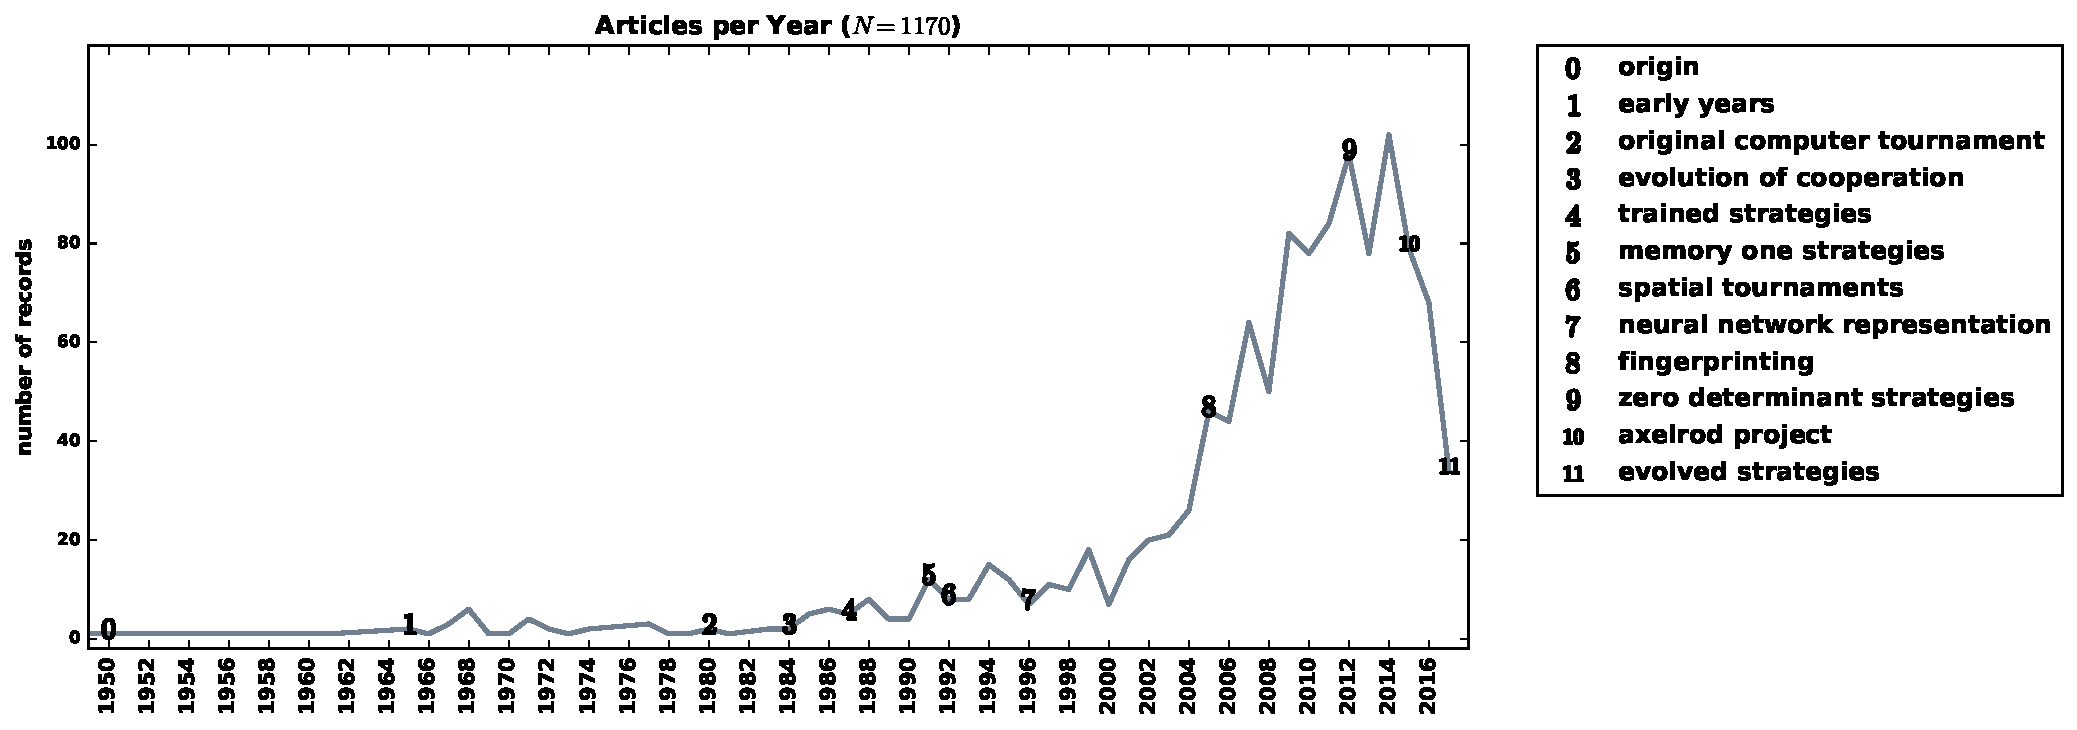
\includegraphics[width=\textwidth]{assets/images/timeline.pdf}
    \caption{\label{fig:timeline} A timeline of the prisoner's dilemma research.}
\end{figure}

\section{Timeline}\label{section:timeline}

\subsection{Origin and (1961-1972)}

The origin of the prisoner's dilemma goes back to the 1950s in early experiments
conducted in RAND~\cite{Flood1958} to test the applicability of games
described in~\cite{VonNeumann1944}. Though in~\cite{Flood1958} the two player game was
introduced the name behind the game was given later the same year.
A. W. Tucker, the PhD advisor of J. Nash, in an attempt to delivery the game
with a story during a talk used prisoners as players and the game is known as
the prisoner's dilemma ever since~\cite{Tucker1983}.

The study of the prisoner's dilemma has attracted people from various fields
across the years. An early figure within the field is Prof A. Rapoport,
a mathematical psychologist, whose work focused on peacekeeping.
In his early work~\cite{rapoport1965} Rapoport conducted experiments using humans
to simulate a play of the prisoner's dilemma. Experimental groups were not been
used only by Rapoport but it was a common mean of studying the game
\cite{Evans1966, Gallo1968, Lutzker1961, Mack1971, Sensenig1972} and are still
being used to date. %TODO reference a good article with human studies.

Those experiments explored the conditions under which altruist behaviour emerges
in human societies. Conditions such as, the gender~\cite{Evans1966,
Lutzker1961, Mack1971} of individuals, the representation of the game
\cite{Evans1966}, the distance between players~\cite{Sensenig1972}, the start effect
\cite{Tedeschi1968} and whether the experimenter was biased~\cite{Gallo1968}.

Even though, several of these experiments were held and continuous research on
the topic was undergoing game theorists were still arguing with each other about
the best way to play the game~\cite{rapoport1965}. Inspired by the work of
Rapoport and intrigued by the very same question the political scientist R. 
Axelrod took upon him to identify the dominant strategy of the prisoners dilemma.
 
The main difference on Axelrod's approach was that machines were going to be used 
instead of humans. The issues with using humans, according to Axelrod
\cite{Axelrod2012}, was the fact that humans can act very randomly even though
the aim of the game is cleared to them. Thus, Axelrod was the first researcher,
to the author's knowledge, to perform a computer tournament of the iterated
prisoner's dilemma. The work of Axelrod is considered one of the greatest
milestones within the field. The tournaments and their results are discussed in
the next session.

\subsection{Axelrod's Tournaments (1981-1984)}\label{subsection:axelrods_tournament}

This section serves as a follow up from the earlier years of the topic and as an
introduction to the modern ways of studying the prisoner's dilemma. It is 
dedicated to the computer tournaments of Axelrod from 1981 to 1984. 

The first computer tournament was performed in 1980~\cite{Axelrod1980a}.
Several scientists were invited to submit their strategies, written in the
programming languages Fortran or Basic. There was a total number 13 submissions
made by the following researchers,

\begin{multicols}{2}
    \begin{enumerate}
        \item T Nicolaus Tideman and Paula Chieruzz;
        \item Rudy Nydegger;
        \item Bernard Grofman;
        \item Martin Shubik;
        \item Stein and Anatol Rapoport;
        \item James W Friedman;
        \item Morton Davis;
        \item Jim Graaskamp;
        \item Leslie Downing;
        \item Scott Feld;
        \item Johann Joss;
        \item Gordon Tullock;
        \item Name not given.
    \end{enumerate}
\end{multicols}

Each strategy competed against all the 13 opponents, itself and a player that played
randomly a match of 200 turns. This topology is called round robin and is the 
equivalent of a complete graph. The tournament was repeated \(5\) times to
reduce variation in the results. Each participant knew the exact length of the
matches and had access to the full history of each match. Furthermore, Axelrod
performed an preliminary tournament and the results were known to the participants.
The payoff values used where \(R=3, P=1, T=5\) and \(S=0\). These values are
commonly used in the literature and unless specified will be the values used in
the rest of the work described here. 

The winner of the tournament was determined by the total average score and not by
the number of matches won. The strategy that was announced the winner was
submitted by Rapoport and was called \textbf{Tit For Tat}. Tit for Tat, is a 
strategy that always cooperates on the first round and then mimics the opponent's
previous move. 

Examples of Tit for Tat interacting with deterministic opponents are given by 
Tables~\ref{table:tft_vs_c}, \ref{table:tft_vs_d}, \ref{table:tft_vs_a}. 
The opponents are, \textbf{Cooperator} a strategy that always cooperates, 
\textbf{Defector} an opponent that always defects and \textbf{Altenator} a 
player who alternates between cooperating and defecting.

\begin{table}[!hbtp]
    \begin{center}
    \begin{tabular}{lcc}
        \toprule
        Turns & Tit for Tat & Cooperator\\
        \toprule
        1 & C & C\\
        2 & C & C\\
        3 & C & C\\
        $\vdots$ & $\vdots$ & $\vdots$ \\
        200 & C & C \\
        \bottomrule
    \end{tabular}
    \caption{Tit for Tat example match against Cooperator}\label{table:tft_vs_c}
    \end{center}
\end{table}

\begin{table}[!hbtp]
    \begin{center}
    \begin{tabular}{lcc}
        \toprule
        Turns & Tit for Tat & Defector\\
        \toprule
        1 & C & D\\
        2 & D & D\\
        3 & D & D\\ 
        $\vdots$ & $\vdots$ & $\vdots$ \\ 
        200 & D & D \\
        \bottomrule
    \end{tabular}
    \caption{Tit for Tat example match against Defector}\label{table:tft_vs_d}
\end{center}
\end{table}

\begin{table}[!hbtp]
    \begin{center}
    \begin{tabular}{lcc}
        \toprule
        Turns & Tit for Tat & Altenator\\
        \toprule
        1 & C & C\\
        2 & C & D\\
        3 & D & C\\ 
        $\vdots$ & $\vdots$ & $\vdots$ \\ 
        200 & C & D \\
        \bottomrule
    \end{tabular}
    \caption{Tit for Tat example match against Altenator}\label{table:tft_vs_a}
\end{center}
\end{table}

The results of the first tournament were filled with surprises. Tit for Tat the
simplest strategy of all had won and had managed to defeat even entrants that
tried to improve on Tit for Tat after the preliminary tournament results. 
Axelrod justified the success of the strategy saying that the strategy was
`nice' and `forgiving'. 

The top eight ranked strategies have been strategies that never defected on the
first round, thus they were described as `nice' strategies. Compared to the rest
nice strategies Tit for Tat had also another property. That property was 
`forgiveness'. Tit for Tat punished it's opponent for a defection but just once
and then it would try to cooperate again.

These two properties were described to be the secret of success in a prisoner's
dilemma tournament. In order to further test the robustness of the results
Axelrod performed a second tournament~\cite{Axelrod1980b}. This time a total of
63 participants submitted strategies for the second tournament, their names were
the following,

\begin{multicols}{3}
    \begin{enumerate}
        \item Gail Grisell;
        \item Harold Rabbie;
        \item James W Friedman;
        \item Abraham Getzler;
        \item Roger Hotz;
        \item George Lefevre;
        \item Nelson Weiderman;
        \item Tom Almy;
        \item Robert Adams;
        \item Herb Weiner;
        \item Otto Borufsen;
        \item R D Anderson;
        \item William Adams;
        \item Michael F McGurrin;
        \item Graham J Eatherley;
        \item Richard Hufford;
        \item George Hufford;
        \item Rob Cave;
        \item Rik Smoody;
        \item John Willaim Colbert;
        \item David A Smith;
        \item Henry Nussbacher;
        \item William H Robertson;
        \item Steve Newman;
        \item Stanley F Quayle;
        \item Rudy Nydegger;
        \item Glen Rowsam;
        \item Leslie Downing;
        \item Jim Graaskamp and Ken Katzen;
        \item Danny C Champion;
        \item Howard R Hollander;
        \item George Duisman;
        \item Brian Yamachi;
        \item Mark F Batell;
        \item Ray Mikkelson;
        \item Craig Feathers;
        \item Fransois Leyvraz;
        \item Johann Joss;
        \item Robert Pebly;
        \item James E Hall;
        \item Edward C White Jr;
        \item George Zimmerman;
        \item Edward Friedland;
        \item X	Edward Friedland;
        \item Paul D Harrington;
        \item David Gladstein;
        \item Scott Feld;
        \item Fred Mauk;
        \item Dennis Ambuehl and Kevin Hickey;
        \item Robyn M Dawes and Mark Batell;
        \item Martyn Jones;
        \item Robert A Leyland;
        \item Paul E Black;
        \item T Nicolaus Tideman and Paula Chieruzz;
        \item Robert B Falk and James M Langsted;
        \item Bernard Grofman;
        \item E E H Schurmann;
        \item Scott Appold;
        \item Gene Snodgrass;
        \item John Maynard Smith;
        \item Jonathan Pinkley;
        \item Anatol Rapoport.
    \end{enumerate}
\end{multicols}

All the participants knew the results of the previous tournament. The rules 
were similar to those of the first tournament with only one exception;
the number of turns was not specified instead a probabilistic ending tournament was
meant to be used. In a probabilistic ending tournament each match has probability 
of ending after each turn. This is  also refereed as `shadow of the future'
\cite{Axelrod1988}.

However, the tournament was not a probabilistic ending one. A fixed probability 
of  0.0036 was chosen as a chance of ending a match with each given move. The
value was chosen so that the expected median length of a match would be 200
turns. The topology was of a round robin and each pair of players was matched 
5 times. The length of the matches was determined once by drawing a random sample.
Each of the five matches had a length of 63, 77, 151 and 308.

The results of the tournament once again came as a surprise. Tit for Tat was the
simplest submission in the second tournament and won the second tournament as well.
Tit for Tat provided proof that reciprocity behaviour can allow cooperation
to emerge in the iterated prisoner's dilemma game. In~\cite{Axelrod1980a}
the main conclusions indicating strong performance was:

\begin{itemize}
    \item that it start of by cooperating
    \item it would forgive it's opponent after a defection
    \item after opponents identified that they were playing Tit for Tat choose
    to cooperate for the rest of the game.
\end{itemize}
%The strategies of the second tournament where bias due the first tournament. Discuss with V. 

Another successful strategy from Axelrod's tournament that can been seen
in literature to date is \textbf{Grudger}. Grudger is a strategy that will cooperate
as long as the opponent does not defect. The name Grudger was give to the strategy
in~\cite{Li2014}. Though the strategy goes by many names in the literature such as,
Spite~\cite{Beaufils1997}, Grim Trigger~\cite{Banks1990} and Grim~\cite{Van2015}.

As for the rest of the strategies, though a full explanation of all 14 strategies
is given in~\cite{Axelrod1980a} the same does not hold for all 63 strategies of
the second tournament~\cite{Axelrod1980b}. The author mainly focuses on the high
ranked participants and several details for the rest strategies are left unknown. 

However, the source code of the 63 strategies be found on Axelrod's personal
website~\cite{fortan_code}. The source code was written by Axelrod and several 
other contributors. The strategies written in Basic were translated to 
Fortran before the tournament. The source code includes the code only for the
strategies and not for creating and performing the tournament.Figure~\ref{fig:tit_for_tat_fortran}
serves as an example of the source code giving the code for the the winning
strategy Tit for Tat. Unfortunately, the source code of the first 13 strategies
is not available, as stated in Axelrod's personal website~\cite{fortan_code}.

\begin{figure}[!hbtp]
    \centering
    \begin{minted}
        [
        autogobble=true,
        framesep=2mm,
        fontsize=\normalsize,
        ]
        {fortran}
    FUNCTION K92R(J,M,K,L,R, JA)
C BY ANATOL RAPOPORT
C TYPED BY AX 3/27/79 (SAME AS ROUND ONE TIT FOR TAT)
c replaced by actual code, Ax 7/27/93
c  T=0
c   K92R=ITFTR(J,M,K,L,T,R)
      k92r=0
      k92r = j
c test 7/30
c   write(6,77) j, k92r
c77   format(' test k92r. j,k92r: ', 2i3)
      RETURN
      END
    \end{minted}
    \caption{\label{fig:tit_for_tat_fortran} Source code for Tit for Tat in Fortran.
    Provided by~\cite{fortan_code}.}
\end{figure}

So far it was discussed how the performance of the strategy was tested through
tournament against other strategies. But is the overall success of a strategy
based only on it's performance in a round robin tournament or should it be
checked through other ways as well?

Following his initial tournaments Axelrod performed an `ecological' tournament
in 1981~\cite{Axelrod1984}. In~\cite{Axelrod1984}, the set of strategies from
Axelrod's second tournament was used to perform the ecological tournament. The
63 strategies interacted generation after generation to a round robin competition
where their frequencies were proportional to their payoff in the previous round.
The ecological approach is based on the payoff matrix of the tournament. The
highest performing strategies are adapted by lower scoring individuals
within a fixed population. Over time a strategy takes over the population.
Figure~\ref{fig:ecological.tournament} demonstrates an example of the
natural selection proceeder. Four different strategies are being used by the
population, Defector, Alternator, TitForTat and Grudger. In~\cite{Axelrod1984},
the results showed that in a homogeneous population of Tit for Tat invasion by
mutant strategies was not successful.

The ability of strategies to be favoured under natural selection and their
ability to withstand invasion from other strategies soon became an new measure
of performance; refereed to as the stability of a strategy.

\begin{figure}[!hbtp]
    \centering
    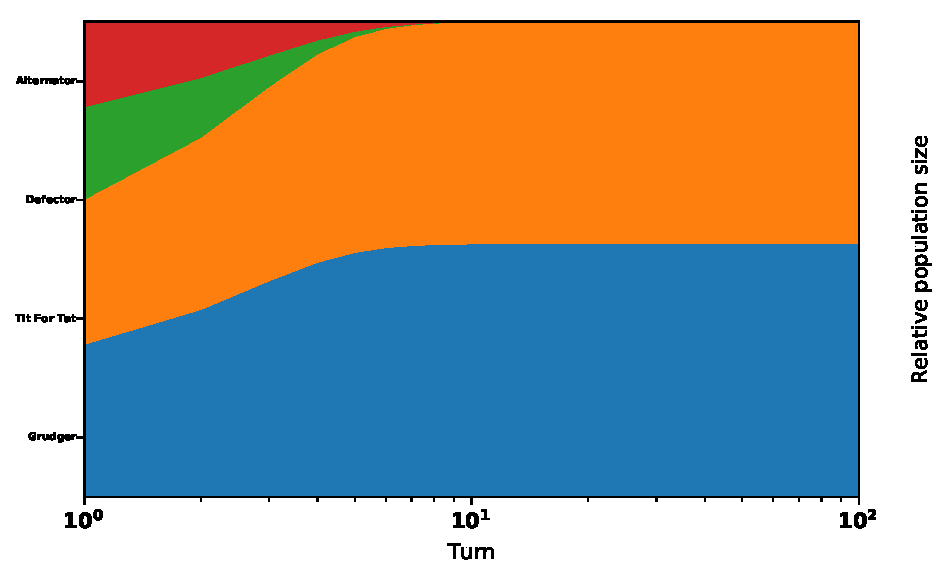
\includegraphics[width=.6\textwidth]{./assets/images/ecological.pdf}
    \caption{System evolving over time based on natural selection using
    \cite{axelrodproject}.}
    \label{fig:ecological.tournament}
\end{figure}

\subsubsection{Immediate work and Criticism on Computer Tournaments (1984-1993)}

The pioneer work of computer tournaments and the results on the reciprocal behaviour
of the prisoner's dilemma spread the knowledge of the game not only worldwide
but also across different scientific principles. The study of cooperation was 
once again a critical issue. This section focuses on the immediate research
that was spawn after the initial computer tournaments and on the criticism these
tournaments received from 1984 to 1993.

Ecological studies that made use of Axelrod's results include the 
works of~\cite{Godfray1992, Milinski1987, Wilkinson1984}. In\cite{Milinski1987}
an experiment was conducted using sticklebacks to test the robustness of the 
strategy Tit for Tat in the interactions of fish. Fish usually travel in pairs
and monitor their hunters to gain information on the enemy. The works of
\cite{Godfray1992, Wilkinson1984} looked upon food sharing between vampire bats.

Nevertheless success often comes with criticism. Axelrod's tournaments assumed that
each player has perfect information of the opponent's actions. In real life
situations this is not always the case. Colleagues' interactions often suffer from
measures of uncertainty. In the original tournaments there was no possibility of
mis implementation or misunderstanding. These stochastic variations are refereed
to as \textbf{noise} and \textbf{mis perception}. Noise is the concept of flipping
one's move based on a given probability. On the contrary, mis perception is the
probability that the opponent's current move is flipped before being recorded.
Noise will flip a player's action  and it will be recorded correctly in the history
where mis perception will not have an effect on the player's move but it will be
recorded wrong~\cite{Hoffmann1998}.

The performance of Tit for Tat was proven to suffer from such stochasticity in
the tournament environment, especially against itself~\cite{Bendor1991, Godfray1992,
Molander1985, Nowak1992}. If two strategies playing Tit for Tat were % Wolfgang2006
to compete against each other in a noisy environment the strategies will get 
a series of unwanted defections. In a non noisy environment
the two strategies would have been cooperating for the entire match.
An interesting result was introduced by~\cite{Molander1985}. Molander stated
that if two strategies playing Tit for Tat meet in a noisy match the average
payoff that a strategy will receive will be the same as that of a Random player
(with probability \(0.5\) of cooperating). 

In~\cite{Bendor1991} a similar tournament to that of Axelrod's was performed 
but this time noise was used. Bendor invited academics to submit strategies 
to participate in his tournament. A total of thirteen strategies were used 
including already existed strategies such as Tit for Tat and \textbf{Tit for Two 
Tats}. The results showed that Tit for Tat performed purely placing eight in
the tournament. Bendor stated that a more forgiving strategy was needed, in his
tournament a strategy called \textbf{Nice and Forgiving} ranked first.

The work of~\cite{Nowak1992} following a similar approach agreed with the result.
In~\cite{Nowak1992}, the space of re-active strategies was explored in a noisy
environment. The strategy that was performing the best in that environment was
the re-active strategy known as \textbf{Generous Tit for Tat}. Reactive strategies
are a subset of memory one strategies introduced in 1989~\cite{nowak1989}.
Reactive strategies are denoted by the probabilities to cooperate after a
\textbf{C} and a \textbf{D} of the opponent. Thus, a reactive strategy only
considers the previous turn of the opponent. Strategies such as, Tit for Tat and
Generous Tit for Tat are reactive.

The author published yet another paper a years later~\cite{Nowak1993} introducing another
interesting player. The new strategy had the tolerance of Generous Tit for Tat 
but also the capability of resisting and invading an all-out cooperators population
was. The strategy is called \textbf{Pavlov}, and is based on the fundamental
behavioural mechanism win-stay, lose-shift. The strategy starts off with a
\textbf{C}, then Pavlov will repeat it's last move it was awarder with by
\(R\) or \(T\) but will shift if punished by \(P\) or \(S\). Palvov is a memory
one strategy.

Memory one strategies, are a set of strategies that consider only the last turn
of the game to decide on the next action~\cite{Nowak1990}. They are represented
by the four conditional probabilities \(p_1, p_2, p_3\) and
\(p_4\) to cooperate after \(CC, CD, DC\) and \(DD\) respectively
(the four possible states a player can be in if only the last turn of the game was
to be considered). Reactive strategies are just a constrained version where
\(p_1=p_3\) and \(p_2=p_1\). The first action of the strategy (when the history
does not exist yet) is assumed to be \textbf{C} unless is stated otherwise. For
example, a reactive strategy called \textbf{Suspicious Tit for Tat}, studied
in~\cite{Nowak1992}.

Other strategies that made an impact have been \textbf{Tit for Two Tats}~\cite{Axelrod1988},
\textbf{Handshake}~\cite{Robson1989} and \textbf{Gradual}~\cite{Beaufils1997}.
Presented in 1988, 1989 and 1997 respectively. Tit for Two Tats, is a variant
of the classic strategy which defects only if the other player defected on the
two preceding moves. Handshake is a strategy that starts with cooperation,
defection. If the opponent plays in a similar way then it will cooperate forever,
otherwise it will defect forever.Gradual starts off by cooperating, then after
the first defection of the other player, it defects one time and cooperates twice.
After the second defection of the opponent, it defects two times and cooperates
twice. After the \(n^{th}\) defection it reacts with \(n\) consecutive defections
and then two cooperations. 

\subsection{Evolutionary Dynamics (1987-1999)}

The results of the round robin tournaments were not the only ones to receive
criticism. Similarly, the ecological tournament and the statements for
the stability of Tit for Tat were also delved into by other researchers.
The results of~\cite{Boyd1987} argued that no pure strategy is evolutionary
stable in the iterated prisoner's dilemma. This was not proven analytically,
instead a series of examples using strategies such as Tit for Tat, Suspicious
Tit for Tat and Defector where explored.

The results were questioned by~\cite{May1987}, stating that much was
still no fully explored and more research had to be put into the results.
Another attempt to explore stability of strategies in the prisoner's dilemma
was done in~\cite{Boyd1989}. This time exploring the results in a noisy
environment, but similarly a analytical proof was not achieved.

An extension to the natural selection was introduced in the 1992~\cite{Nowak1992b},
recommending a different type of topology. A population of two deterministic
strategies, Defector and Cooperator, were placed on a a two dimensional square array
where the individuals could interact only with the immediate neighbours.
The number of immediate neighbours could be either, fourth, six or eight. As
shown in Figure~\ref{fig:topologies}. The authors claimed that the essential
results remain true of all topologies; the results also hold whether self interactions
are taken into account.

Thus each cell of the lattice is occupied by a \textbf{C} or a \textbf{D} and in
each generation step each cell owner interacts with its immediate neighbours and
play the game. The score of each player is the sum of the overall games the player
competed in. At the start of the next generation, each lattice cell is occupied by the
player with the highest score among the previous owner and the immediate
neighbours. Nowak and all created this model where the model parameter
has been the temptation payoff denoted as \(b\). Thus \(T=b\). For 
different values of the parameter \(b\) it was shown that cooperators and
defectors can persist together indefinitely. This topology is refereed to as
spatial topology.

\begin{figure}[!hbtp]
\centering
    \begin{subfigure}{.25\textwidth}
        \hspace{.8cm}
        \includestandalone[width=0.6\textwidth]{assets/tex/neighb_four}    
    \end{subfigure}
    \begin{subfigure}{.25\textwidth}\centering
        \includestandalone[width=0.6\textwidth]{assets/tex/neighb_eight} 
     \end{subfigure}
     \begin{subfigure}{.25\textwidth}\centering
        \includestandalone[width=0.6\textwidth]{assets/tex/neighb_six} 
     \end{subfigure}
    \begin{subfigure}{.25\textwidth}
        \includestandalone[width=\textwidth]{assets/tex/square_lattice}    
    \end{subfigure}
    \begin{subfigure}{.25\textwidth}\centering
        \includestandalone[width=\textwidth]{assets/tex/square_lattice_eight} 
     \end{subfigure}
     \begin{subfigure}{.25\textwidth}\centering
        \includestandalone[width=\textwidth]{assets/tex/hexagonal_lattice} 
     \end{subfigure}
     \caption{Spatial neighbourhoods}\label{fig:topologies}
    \end{figure}

Evolutionary dynamics have been highly useful in the research of the prisoner's
dilemma. In~\cite{Axelrod1987}, an evolutionary process, called the genetic
algorithm, was used to discover effective strategies. The author introduced
lookup tables as a mean of representing a strategy in a gene format. A lookup
table is a set of deterministic responses based on the opponents \(m\) last
moves; \cite{Axelrod1987} considered \(m=3\).

\subsection{Modern approaches (1995-2015)}\label{section:modern_approaches}

This section covers several pieces of work from 1995 to 2015. During this time
period several aspects discussed in the previous sections are now being applied
continuously and are considered standard means of researching the iterated
prisoners dilemma.

Several computer tournaments are performed, and new strategic rules surface.
The performance of these strategic rules is being measured by round robin tournaments
and evolutionary tournaments.
 
A number of Tit for Tat variants make an appearance and are introduced as more
as more dominant than Tit for Tat. These include, \textbf{Contrite Tit for Tat}
\cite{Wu1995} and \textbf{Adaptive Tit for Tat}~\cite{tzafestas-2000a}.
On the other hand, defector variants have also been studied~\cite{Hilde2013}.
\textbf{Anti Tit for Tat}, is a strategy that plays the opposite of the opponents
previous move. Another limitation of the strategy was discussed in~\cite{Wolfgang2006}.
Tit for Tat was proven to hit a deadlock. Deadlock meaning a loop between 
cooperation and defection. \textbf{Omega Tit For Tat} was introduced and was
a strategy capable of avoiding the deadlock~\cite{Wolfgang2006}.

In 2011 the authors of~\cite{Li2011} performed their own tournament where 
several interesting strategies made an appearance.

\begin{itemize}
    \item \textbf{Periodic player CCD}, plays \textbf{C}, \textbf{C}, \textbf{D} 
    periodically. Note that variations of a period player also make appearance
    in the article but will not be listed here.
    \item \textbf{Prober}, starts with the pattern \textbf{D}, \textbf{C}, \textbf{C}
     and then defects if the opponent has cooperated in the second and third move;
     otherwise, it play as Tit for Tat.
    \item \textbf{Reverse Pavlov}, a strategy that does the reverse of Pavlov.
\end{itemize}

In earlier work the same author introduced a strategy called \textbf{APavlov},
which stands for adaptive Pavlov~\cite{Li2007}. The strategy attempts to 
classify the opponent as one of the following strategies, All Cooperator, 
All Defector, Pavlov, Random or \textbf{PavlovD}. PavlovD, is just Pavlov
but it starts the game with a \textbf{D}. Once Adaptive Pavlov has classified
the opponent plays to maximize it's payoff.

Evolutionary dynamics and optimization methods are used with different representation
methods in order to discover new optimized strategies. Include lookup tables
\cite{Axelrod1987, Lindgren1994}, artificial neural networks~\cite{Fogel1996,
Lee2015} and finite state machines~\cite{Miller1996, Rubinstein1986}.

Strategies based on finite state machines are described by the number of states.
The strategy selects the next action in each round based on the current state
and the opponent's last move, transitioning to a new state each time. Figure~\ref{fig:tit_for_tat_fsm},
illustrates the finite state representation of Tit For Tat.

\begin{figure}[!hbtp]
    \centering
    \includestandalone[width=.3\textwidth]{./assets/tex/tit_for_tat_fsm}
    \caption{Finite state machine representation of Tit for Tat.}
    \label{fig:tit_for_tat_fsm}
\end{figure}

In~\cite{Ashlock2006b} the author presented two new strategies that have
been trained using a finite state machine representation. They are called,
\textbf{Fortress3} and \textbf{Fortress4}. Figure~\ref{fig:fortress3_and_4}
illustrates their diagrammatic representation where the transition arrows are 
labelled \textit{O/P} where \textit{O} is the opponent's last action and \textit{P}
is the player's response.

\begin{figure}[!hbtp]
\centering
    \begin{subfigure}{.4\textwidth}
        \includestandalone[width=\textwidth]{assets/tex/fortress_3}
    \end{subfigure}
    \begin{subfigure}{.4\textwidth}\centering
        \includestandalone[width=\textwidth]{assets/tex/fortress_4}
     \end{subfigure}
     \caption{Representations of Fortress 3 and Fortress 4. Note that the
     strategy's first move, enters state 1, is defection for both strategies.}
     \label{fig:fortress3_and_4}
\end{figure}

Optimisation methods will return a spectrum of strategies. In order to distinguish
the strategies and assuring that they are indeed different \cite{Ashlock2005} 
introduced a method called fingerprinting. 

The method of fingerprinting is a technique for generating a functional signature for a 
strategy~\cite{Ashlock2008}. This is achieved by computing the score of a strategy
against a spectrum of opponents. The basic method is to play the strategy
against a probe strategy with varying noise parameters. In~\cite{Ashlock2005} 
Tit for Tat is used as the probe strategy. Fingerprint functions
can then be compared to allow for easier identification of similar strategies.
In Figure~\ref{fig:fingerprinting} an example of Pavlov's fingerprint is given.
Fingerprinting has been studied in depth in~\cite{Ashlock2008, Ashlock2009, 
Ashlock2010, Ashlock2006a}.

\begin{figure}[!hbtp]
    \centering
    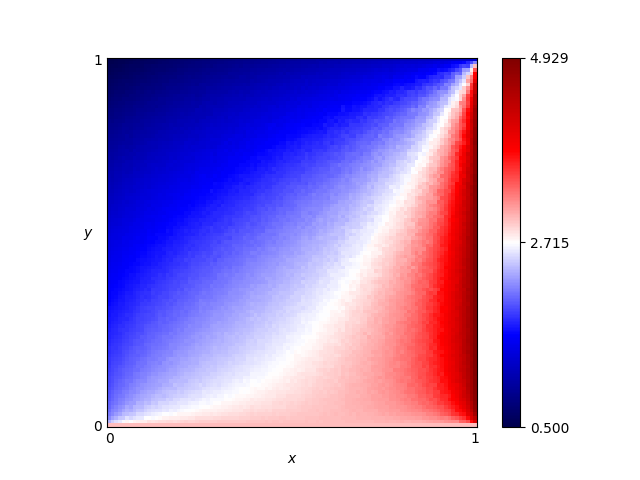
\includegraphics[height=.3\textheight]{./assets/images/Win-Stay_Lose-Shift.png}
    \caption{Pavlov fingerprinting with Tit for Tat used as the probe strategy.
    Figure was generated using~\cite{axelrodproject}.}
    \label{fig:fingerprinting}
\end{figure}

Due the nature of the research several pieces of software are starting to appear,
this includes a library called PRISON~\cite{prison}. PRISON is written in the
programming language Java and it has been used by it's authors in several
publications. The project includes a good number of strategies from the 
literature but unfortunately the last update of the project dates back in 2004.

\subsection{Zero determinant (2012 - 2015)}

Following Section~\ref{section:modern_approaches}, this section is a review
of an important set of strategies, the zero determinant. 

In~\cite{Press2012}, a new set of memory one strategies were introduced, called
\textbf{zero determinant (ZD)} strategies. The ZD strategies,
manage to force a linear relationship between the score of the strategy
and the opponent. Press and Dyson, prove their concept of the ZD strategies
and claim that a ZD strategy can outperform any given opponent.

The ZD strategies have attracted a lot of attention. It was stated that
``Press and Dyson have fundamentally changed the viewpoint on the Prisoner's
Dilemma''~\cite{Stewart2012}. In~\cite{Stewart2012}, a new tournament was
performed including ZD strategies and a new set of ZD 
strategies the \textbf{Generous ZD}. Even so, ZD and memory one strategies have
also received criticism. In~\cite{Lee2015}, the `memory of a strategy does
not matter' statement was questioned. A set of more complex strategies,
strategies that take in account the entire history set of the game, were
trained and proven to be more stable than ZD strategies.

\subsection{Current area (2015 - 2017)}

Following a discussion on research of short memory strategies this section
reviews recent work done in complex strategies. As well as a discussion of
new software and how modern approaches allows us to now revisit several pieces of
work produced in the past.

Modern approaches of artificial neural networks and machine learning are now used
in the field.  A number of strategies based on artificial neural networks are
introduced by~\cite{Knight2017}. Artificial neural networks provide a mapping
function to an action based on a selection of features computed from the history
of play.
 
These strategies are refereed to as \textbf{EvovlvedANN} strategies and are
based on a pre-trained neural network with the following features,

\begin{multicols}{2}
    \begin{itemize}
        \item Opponent's first move is C
        \item Opponent's first move is D
        \item Opponent's second move is C
        \item Opponent's second move is D
        \item Player's previous move is C
        \item Player's previous move is D
        \item Player's second previous move is C
        \item Player's second previous move is D
        \item Opponent's previous move is C
        \item Opponent's previous move is D
        \item Opponent's second previous move is C
        \item Opponent's second previous move is D
        \item Total opponent cooperations
        \item Total opponent defections
        \item Total player cooperations
        \item Total player defections
        \item Round number
    \end{itemize}
\end{multicols}

A representation of \textbf{EvovlvedANN 5} is given in Figure~\ref{fig:ann_5_neural}. 
The inputs of the neural network are the 17 features as listed above. Number 5 
reefers to the size of the hidden layer.

\begin{figure}[!hbtp]
    \centering
    \includestandalone[width=.5\textwidth]{./assets/tex/ann_5_neural}
    \caption{Neural network representation of EvovlvedANN 5.}
    \label{fig:ann_5_neural}
\end{figure}

In~\cite{Knight2017}, these representing methods are refereed to as archetypes.
Finite state machines and artificial neural networks are included in the
work but also new archetypes are introduced, such as hidden Markov models. A variant
of a finite state machine that use probabilistic transitions based on the prior
round of play to other states and cooperate or defect with various probabilities
at each state. Finite state machines and hidden Markov models 
based strategies are characterized
by the number of states. Similarly, artificial neural networks based players
are characterized by the size of the hidden layer and number of input features.

Additionally a variant of a look up table is also presented called the lookerup 
archetype. The lookerup archetype responses based on the opponent's first \(n_1\)
moves, the opponent's last \(m_1\) moves, and the players last \(m_2\) moves.
Taking into account the initial move of the opponent can give many insights. 
For it is the only move a strategy is truly itself without being affected by
the other player. As a reminder, Axelrod in his work 
highlighted the importance of the initial move and believed that it was one
of the secrets of success of the strategy Tit for Tat.

Finally, a new archetype called the Gambler is also introduced, which is a 
stochastic variant of the lookerup archetype.

Archetypes are used with evolutionary algorithms to train set of 
new strategies. The evolutionary algorithm used in both~\cite{Axelrod1987,
Gaudesi2016} is called genetic algorithm. Other algorithms including particle
swarm optimization have been used in research of the most dominant strategy
\cite{Franken2005}.

In~\cite{Knight2017} the approach in used to introduce as stated
by the authors the best performing strategies for the iterated prisoner's dilemma.
These strategies will be refereed  as \textbf{Evolved} strategies.
Several successful new strategies are,

\begin{itemize}
    \item \textbf{EvolvedLookerUp2\_2\_2} a looker up strategy trained with a
    genetic algorithm; EvolvedLookerUp2\_2\_2 responses based on the opponent's 
    2 first and last moves and the player's 2 last moves. Thus \(n_1=2, m_1=2\)
    and \(m_2=2\). 
    \item \textbf{Evolved HMM 5} a 5 states hidden markov model trained with a genetic 
    algorithm;
    \item \textbf{Evolved FSM 16} a 16 state machine trained with a genetic
    algorithm; 
    \item Finally \textbf{PSO Gambler 2 2 2} a looker up strategy trained with
    a particle swarm algorithm, where \(n_1=2, m_1=2\) and \(m_2=2\).
\end{itemize}

Though several papers have claimed before to have discovered the dominant
strategies for the game the work of \cite{Knight2017} is promising. 
This is due the fact that the introduced strategies have been trained using
different types of evolutionary algorithms in a pool of 176 well known 
strategies for the literature. Including all the strategies that have been 
discussed in this section.

This was made possible due an open source  library, called the Axelrod project
\cite{axelrodproject}. The project is written in the programming language 
Python, it is accessible and open source. To date the list of strategies implemented
within the library exceed the 200. The project has been used in several
publications including~\cite{Knight2017} and a paper describing it and
it's capabilities was published in 2016~\cite{Knight2016}. The source code
for Tit for Tat as implement within the library is shown in Figure
\ref{fig:tit_for_tat_axelrod}. Furthermore, performing a tournament 
with a selection of strategies is possible in five lines of code, shown in 
Figure~\ref{fig:tournament_code}.

\begin{figure}[!hbtp]
    \centering
    \begin{minted}
        [
        autogobble=true,
        framesep=2mm,
        fontsize=\normalsize,
        ]
        {python}
def strategy(self, opponent: Player) -> Action:
    """This is the actual strategy"""
    # First move
    if not self.history:
        return C
    # React to the opponent's last move
    if opponent.history[-1] == D:
        return D
    return C
    \end{minted}
    \caption{\label{fig:tit_for_tat_axelrod} Source code for Tit for Tat in Python
    as implemented in Axelrod Python library~\cite{axelrodproject}}.
\end{figure}

\begin{figure}[!hbtp]
    \centering
    \begin{minted}
        [
        autogobble=true,
        framesep=2mm,
        fontsize=\normalsize,
        ]
        {python}
>>> import axelrod as axl
>>> players = (axl.Cooperator(), axl.Defector(), axl.TitForTat(), axl.Grudger())
>>> tournament = axl.Tournament(players)
>>> results = tournament.play()
>>> results.ranked_names
['Defector', 'Tit For Tat', 'Grudger', 'Cooperator']
    \end{minted}
    \caption{\label{fig:tournament_code} Performing a computer tournament
    using~\cite{axelrodproject}.}
\end{figure}

Software has a crucial role in research. Well written and maintained software
allows the reproducibility of prior work and can accelerate findings within the
field. The field of the iterated prisoner's dilemma has suffered the consequences
of poor research software. As stated above the source code of the initial
computer tournament is not retrievable. Several of the strategies that competed
in the tournament are not given a full explanation of how the decided on their
next move. In terms of best practice and reproducibility the Axelrod library
is the lead software in the field.

Other recent projects include~\cite{pd_trust, pd_game}, both are education 
platforms and not research tools. In~\cite{pd_trust}, several concepts such as 
the iterated game, computer tournaments and evolutionary dynamics are introduced
through a user interface game. Project~\cite{pd_game} offers a big collection of
strategies and allows the user to try several match and tournaments configurations.
Such as noise. 

In~\cite{Rapoport2015}, the authors claim that they have managed to 
re-run the first tournament that Axelrod performed. They tried to push his work
further by altering aspects such as, the format of the tournament, the objective
and the population. One of the authors claimed to have been a contributor
to the first tournaments, which would explain how it was managed to reproduce
the tournament.

\subsubsection{Biological Applications}
%TODO include the cancer studies.
\begin{itemize}
    \item \cite{Turner1999} uses evolutionary game theory to study the spread of
    virus.
    \item \cite{Douglas2011} a shout for his work, using tit for tat to study cells.
\end{itemize}

\section{Analysis}\label{section:analysis}

This section follows a circumstantial review of the prisoner's dilemma timeline
conducted by the authors. The section focuses on the analysis of the 
prisoner's dilemma timeline using a large dataset of prisoner's dilemma articles'
metadata. Using various machine learning techniques the number and topics that
have been researched over the years within the field are discussed. Moreover, we 
explore the connections of the authors that have work on the game using
network theory.

\subsection{Data Collection}

Academic articles are accessible through scholarly databases and collections of
journals. Several databases and collections today offer access through an open 
Api. An Api is an application protocol interface that allows users to talk
directly the database, skipping the user interface side of a journal.
Interacting with the Api has two phases:

\begin{itemize}
    \item requesting;
    \item receiving;
\end{itemize}

The requesting phase includes composing a url with the requesting message.
The head of the url includes the address of the Api and the tail the search 
argument, such as the word `prisoner' to exists within the title. The address 
of the Api and the search arguments themselves differ from journal to journal, 
thus different journals can generate complete different requesting urls. 

The second phase of the receiving includes receiving a number of raw metadata of
articles that satisfied the request. The answer is commonly received in an xml
format but similarly the number of features and the syntax of the xml file 
differs from journal to journal.

Data collection is a crucial proceeder. We wanted to include a large number of
articles from various journal for the analysis to be objective. Moreover, we 
wanted the data to be collected within a short period of time. For these reasons
an open source library was developed for the purpose of this work. The library
is called Arcas and though the package it self will not be analysed here the 
source code can be found here, \url{https://github.com/Nikoleta-v3/Arcas}. 

Arcas serves as a translator between us and various Apis. More specifically it
works in coordinate with five different journal. For Arcas to collect data a series
of keywords had to be specified. Each keyword individually is checked weather
it exists within the title or the abstract of an article. Only if this check is
satisfied an article is collected. A list of the keywords that were used in this
work are given by Table~\ref{table:search_keywords}.

\begin{multicols}{3}
    \begin{enumerate}
        \item arXiv;
        \item PLOS;
        \item IEEE;
        \item Nature;
        \item Springer.
    \end{enumerate}
\end{multicols}

\begin{table}[!hbtp]
    \begin{center}
        \begin{tabular}{lll}
            \toprule
             & Keywords & \\
            \midrule
             1 &  prisoner's dilemma & \\
             2 &  prisoners dilemma  & \\
             3 &  prisoners evolution & \\
             4 &  prisoner game theory & \\
             5 &  R Axelrod & \\
             6 &  memory one strategy & \\
             7 & tit-for-tat & \\
             8 & tit for tata & \\
             9 & zero determinant strategies & \\
            \bottomrule
        \end{tabular}
    \end{center}
    \caption{Keywords used in searching for articles.}
    \label{table:search_keywords}
\end{table}

Each entry retrieved by Arcas is constituted of various features which are 
listed on Table~\ref{table:arcas_results}. In the following section only a number
are considered. These are listed on Table~\ref{table:result_set}.

\begin{table}[!hbtp]
    \begin{center}
    \resizebox{0.9\linewidth}{!}{\arraycolsep=2.5pt%
        \begin{tabular}{lll}
            \toprule
             & Result name & Explanation \\
             \midrule
             1 & Abstract & The abstract of the article.\\ 
             2 & Author & A single entity of an author from the list of 
             authors of the respective article.\\ 
             3 & Date & Year of publication.\\ 
             4 & Journal & Journal of publication.\\  
             5 & Key & A generated key containing an authors name and 
             publication year (ex. Glynatsi2017).\\                 
             6 & Keyword & A single entity of a keyword assigned to the article 
             by the given journal.\\ 
             7 & Labels & A single entity of labels assigned to the article 
             manual by us.\\                  
             8 & Pages & Pages of publication.\\               
             9 & Provenance & Scholarly database for where the article was 
             collected.\\                  
             10 & Score & Score given to article by the given journal.\\       
             11 & Title & Title of article.\\               
             12 & Unique key &  A unique key. \\ 
            \bottomrule
        \end{tabular}}
    \end{center}
    \caption{Metadata for each entry/article.}
    \label{table:arcas_results}
\end{table}

\begin{table}[!hbtp]
    \begin{center}
        \begin{tabular}{lll}
            \toprule
             & Result name & Explanation \\
             \midrule
             1 & Abstract & The abstract of the article.\\ 
             2 & Author & A single entity of an author from the list of 
             authors of the respective article.\\ 
             3 & Date & Year of publication.\\ 
             4 & Journal & Journal of publication.\\               
             5 & Provenance & Scholarly database for where the article was 
             collected.\\                        
             6 & Title & Title of article.\\               
            \bottomrule
        \end{tabular}
    \end{center}
    \caption{Structure of data set. Contained results.}
    \label{table:result_set}
\end{table}

\subsection{Preliminary Analysis}

The data set is consisted by a total of \totalarticles articles, although only
\uniquetitles are unique titles. This is because a total of \numberofduplicates
articles have been collected from more than just one Api. All \numberofduplicates
duplicates are from the pre print server arXiv and will be dropped
for the analysis, thus hereupon we consider \uniquetitles entries. The full
data set has been archived and is available online. % archived articles

Though Arcas was used as an automated data collection in progress of writing the
literature review of Section~\ref{section:timeline} the authors have discussed 
a number of articles that were not retrieved by Arcas. This is only because these
articles were not published by the 5 journals considered in the analysis. Even so,
the meta data of those article have been manually included, more specifically
\manual entries. The provenance of the articles are given by Table~\ref{table:provenance}.

More specifically, a total number of 470 articles have been collected from arXiv,
312 from Springer and 241 from IEEE. A smaller number of entries were
contributed by Nature and PLOS.

\begin{table}[!hbtp]
    \begin{center}
    \begin{tabular}{lrr}
\toprule
{} &  \# of Articles &  Percentage \\
provenance &                &             \\
\midrule
Manual     &             89 &        2.92 \\
IEEE       &            295 &        9.67 \\
Springer   &            458 &       15.01 \\
PLOS       &            482 &       15.79 \\
Nature     &            673 &       22.05 \\
arXiv      &           1055 &       34.57 \\
\bottomrule
\end{tabular}

    \end{center}
    \caption{Keywords used in searching for articles.}
    \label{table:provenance}
\end{table}

The eldest entry was published in 1944 and the most recent one in 2017. Note
that the last time data were collected was on December 2017. The provenance of
articles can also be viewed over the year of publication. This is illustrated
in Figure~\ref{fig:provenance}. This allow us to view the significance of each
journal's contribution to the field over the years as well as when the prisoner's
dilemma fitted the scope of each journal. 

Springer and IEEE are the two journals that have been publishing papers on the 
topic for the longest time. Even so, it can been seen that IEEE contributed more
than 10 articles per year after 2002. Similarly, arXiv contributes with a big
number of papers with an increasing trend after the 2000s. Both arXiv and IEEE
are associated with computer engineering and allied disciplines. As a reminder
from Section~\ref{section:timeline}, the `Modern Area' started near the 2000s
where now the study of the prisoner's dilemma is associated with computer science.
PLOS journal was launched on 2000 and it can been seen that accepted it's first
publication on the topic on 2006 and Nature has a few publications over the
years. Nature began it's publications after the work of Axelord in 1980s and
some of it's first publications include the work of Martin Nowak done in the 
1990's.

\begin{figure}[!hbtp]
    \centering
    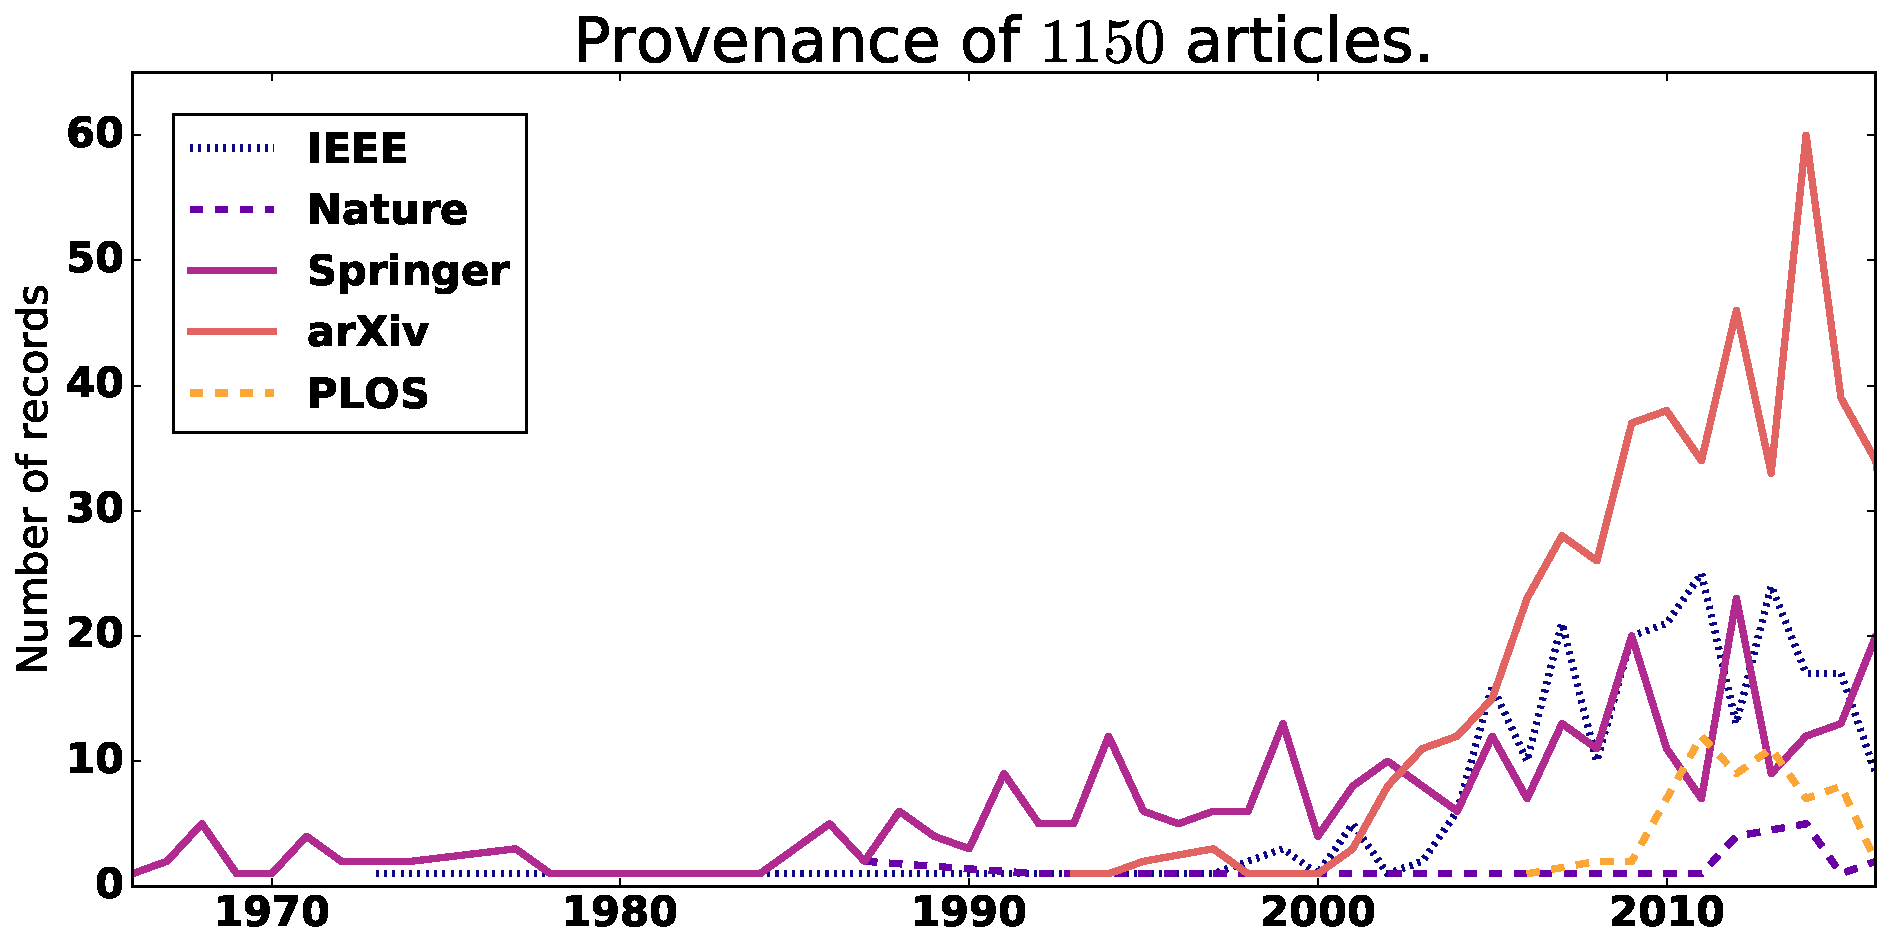
\includegraphics[width=.6\textwidth]{./assets/images/provenance.pdf}
    \caption{Provenance of articles}
    \label{fig:provenance}
\end{figure}

Now that the number and the years over when publications have been made on 
the prisoner's dilemma have been discussed on the following section the people 
that have written about the game and their connections are explored.

\subsection{Authors Analysis}

\subsubsection{Co authors network}
Number of authors varies per paper. Some fields are more collaborative than others.
In this section the connectivity of the authors within the prisoner's dilemma
field is examined. Over the \uniquetitles articles within the data set the total
number of unique authors is \authors.

Note that the authors names had to be cleaned before the analysis could be held.
Several journals use different methods of writing an author's name. For this reason
the Levenshtein Distance was used to calculated the difference between name 
entries. A manual check was performed before replacing the flagged entries
by the Levenshtein Distance.

The authors will be represented in a network. The network, shown in Figure
\ref{fig:authors_network}, has sets of vertices \(V\) and edges \(E\). The 
\authors vertices represent each of the unique authors. The vertices are connected
with an edge if and only if two authors have written together. Weights have been
applied to both the vertices and the edges. Vertices' weight corresponds to 
the number of papers the author has within the data set and the edge weight
to the number of times the authors wrote together. The weighted network can be
seen in Figure~\ref{fig:authors_network_weighted}.

In Figure~\ref{fig:authors_network} it can bee seen that overall the authors 
network is disjoint. Several researchers on the outer circle seem to have written
alone or have a single connection to another researcher. On the other hand,
in the inner circle of the network some connectivity of the vertices does seem
to exists, with a single large cluster located in the middle of the network.
 
More insights can be gained by observing Figure~\ref{fig:authors_network_weighted}
as well. The authors that cover the outer space, that seem to be less collaborative,
are not authors that have single contributions to the field. On the other hand
authors that have repeatedly published on the topic are located in both the outer
and inner circles of the network. 

\begin{figure}[!hbtp]
    \centering
    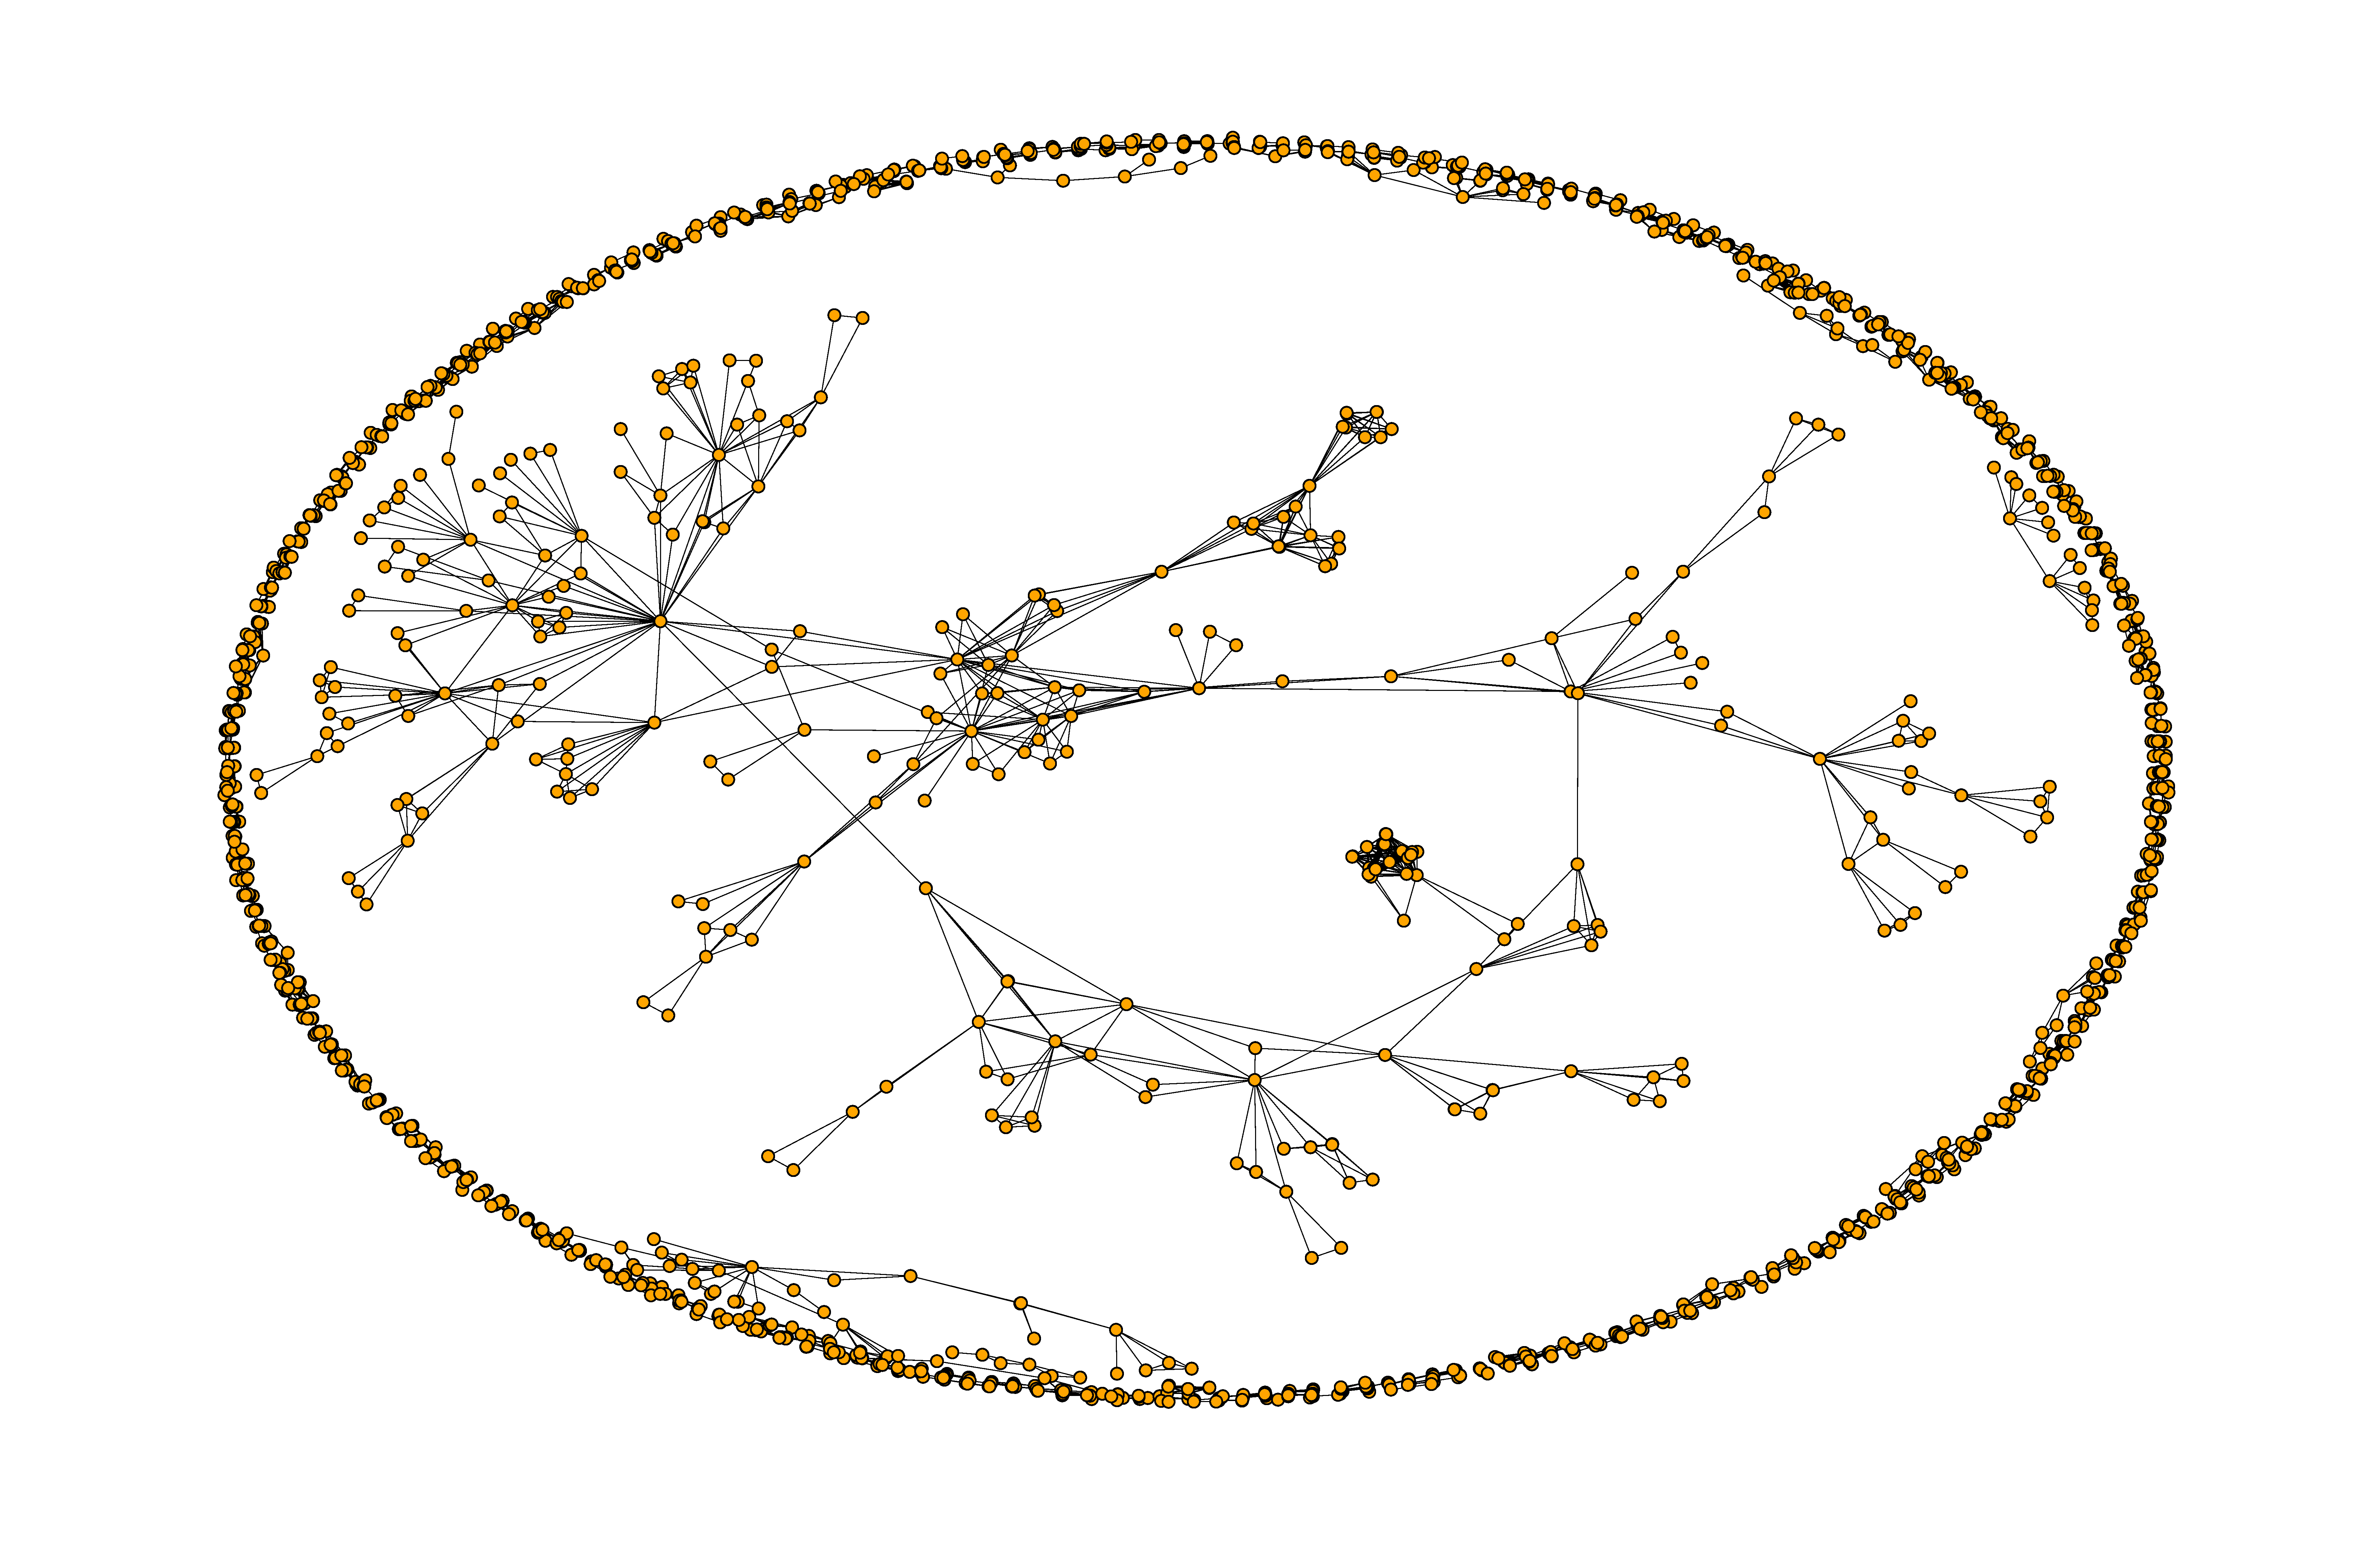
\includegraphics[width=\textwidth]{./assets/images/co-authors-network.pdf}
    \caption{Co authors network.}\label{fig:authors_network}
\end{figure}

\begin{figure}[!hbtp]
    \centering
    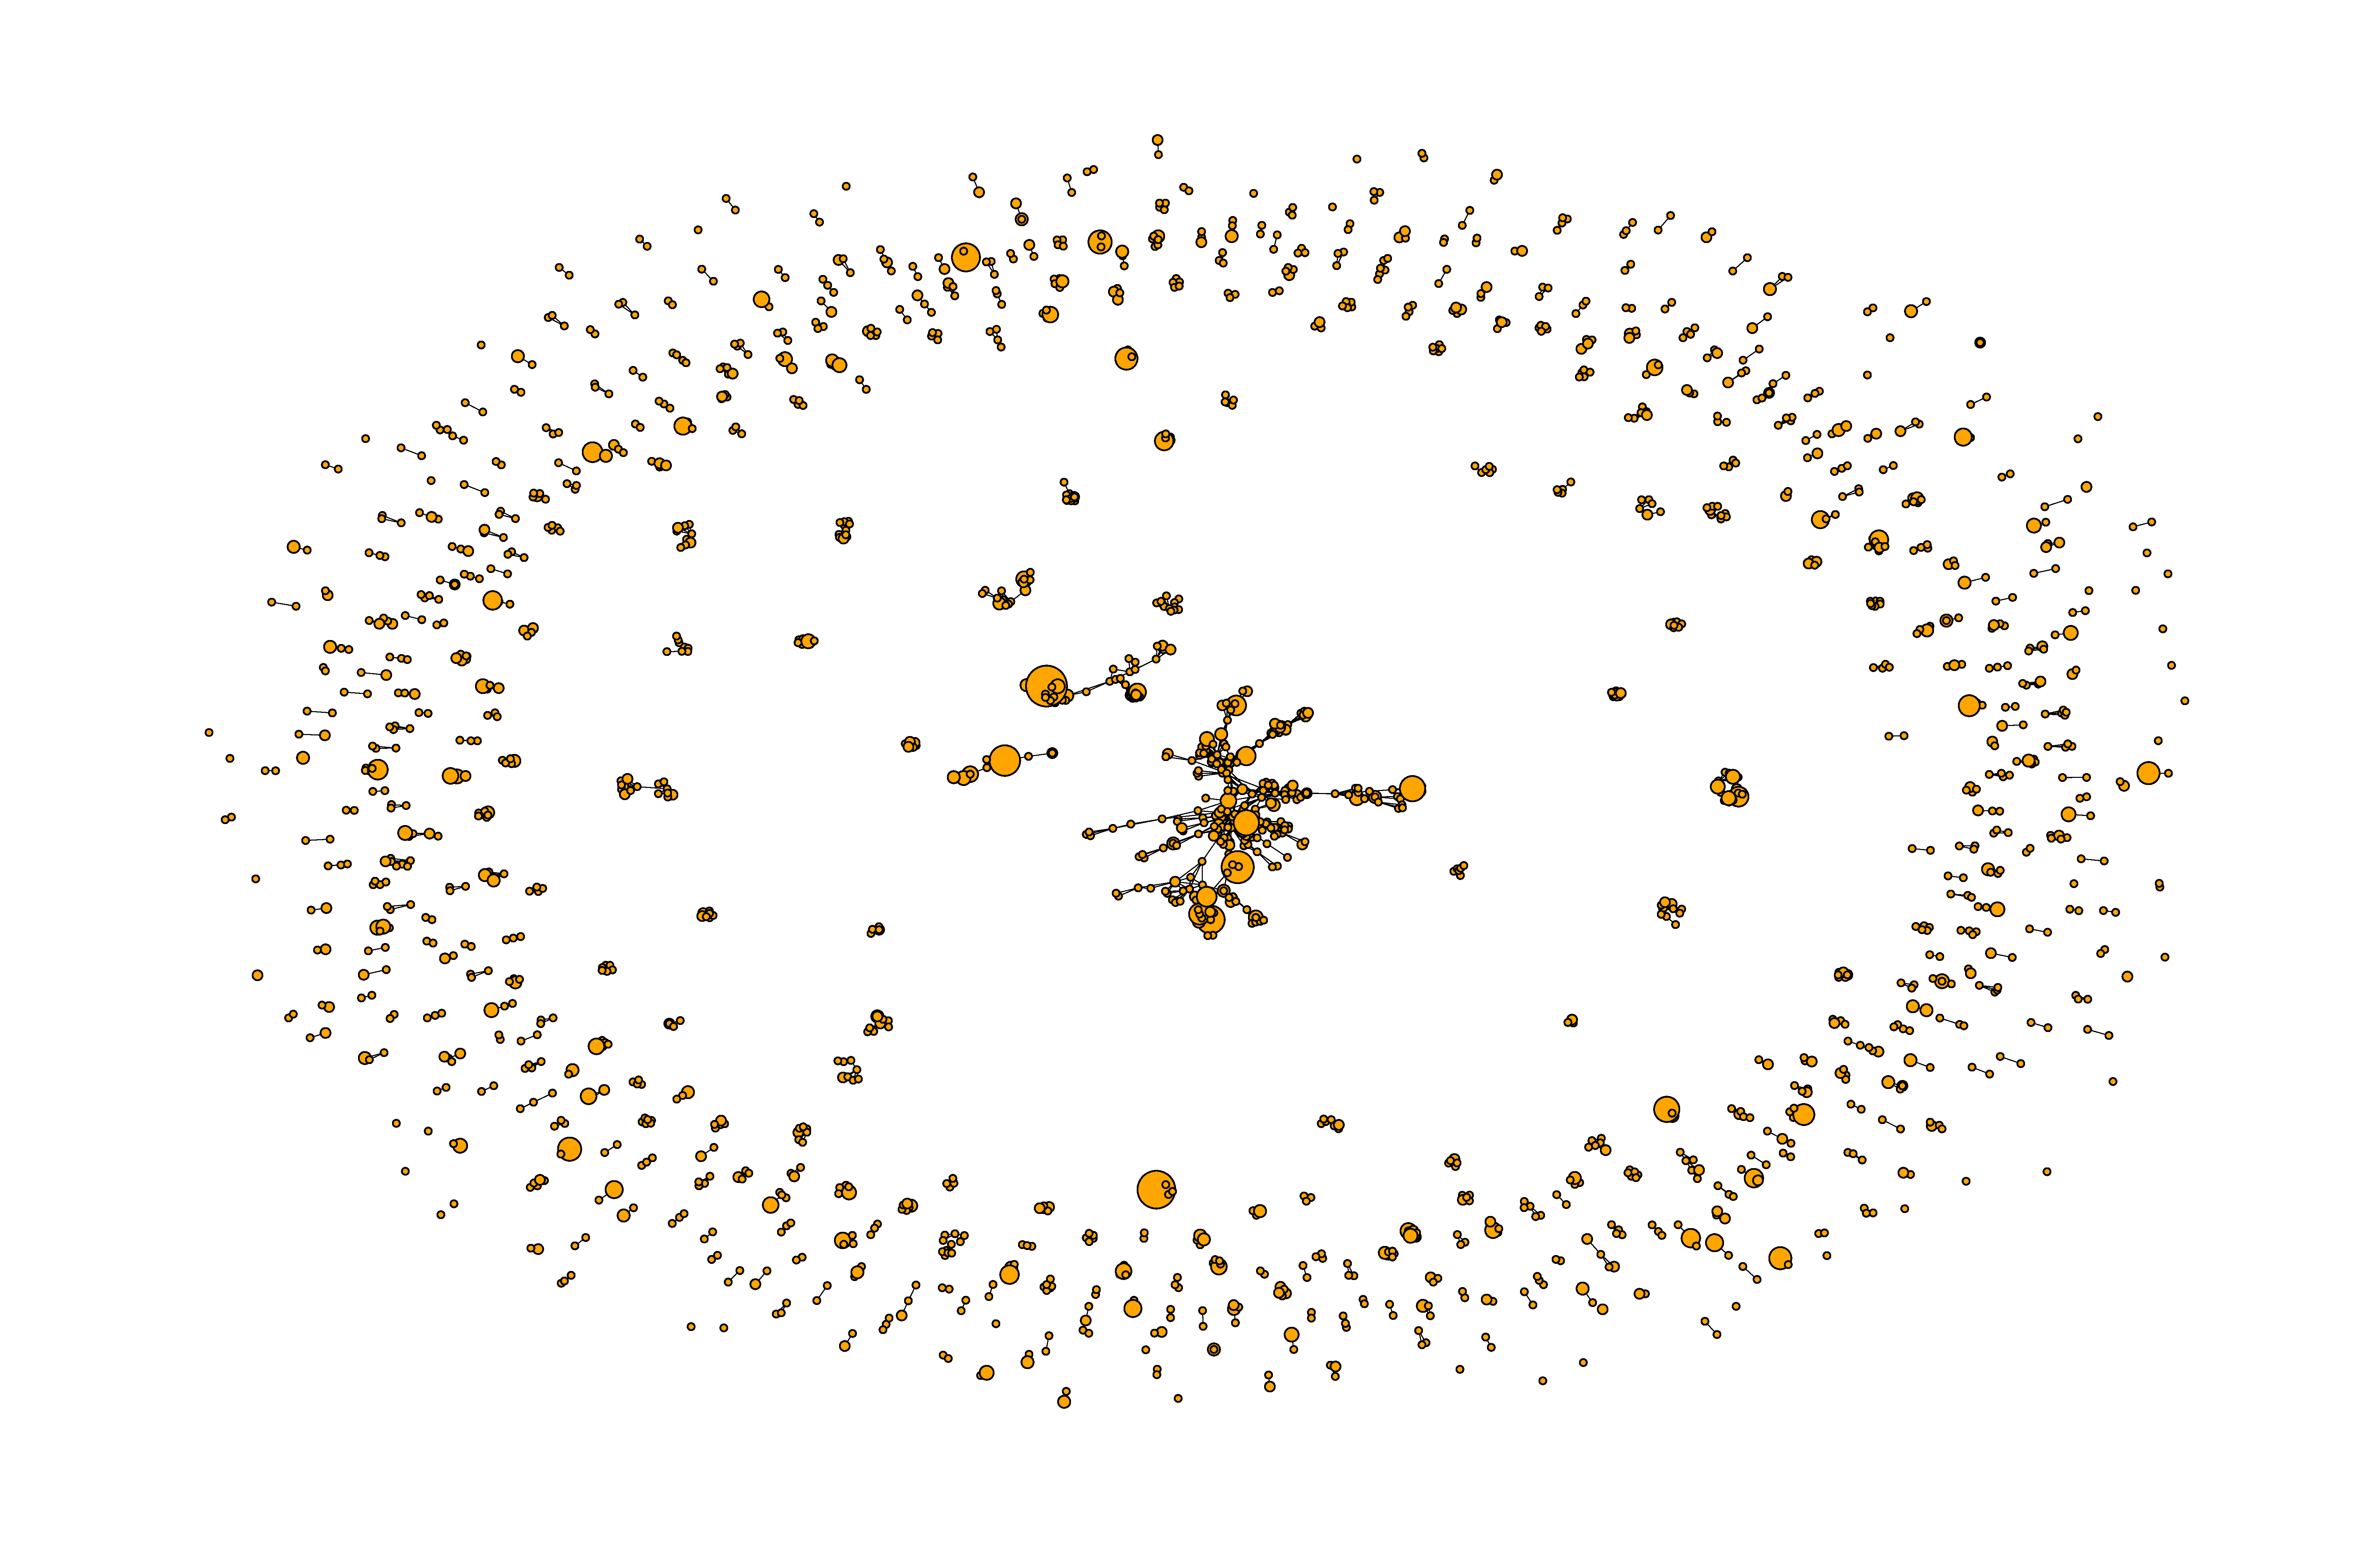
\includegraphics[width=\textwidth]{./assets/images/co-authors-network-weight.pdf}
    \caption{Co authors network with vertices' weight.}
    \label{fig:authors_network_weighted}
\end{figure}

Let's identify the authors with the maximum number of publication in the data set.
The 10 most published authors of the data set are given by Table
\ref{table:most_published}. Authors such as M. Nowak and D. Ashlock, that have
previously been discussed in Section \ref{section:timeline}, appear on the list.
Though other authors such as R. Axelrod do not. On the other hand, several people
whose work was not discussed in the previous section appear here for example 
Matjaz Perc with a total of 34 articles.

The number of publications is not the only measure examined here. The
centrality of the authors is explored in a similar manner. Several measures of
centrality are used in network theory. For the purpose of this work the measure 
examined is the betweenness centrality. The results are given by Table
\ref{table:central_authors}.

\begin{table}[!hbtp]
    \begin{center}
    \begin{tabular}{lr}
\toprule
{} &  unique\_key \\
author          &             \\
\midrule
martin a. nowak &          11 \\
hisao ishibuchi &          13 \\
yamir moreno    &          13 \\
zhen wang       &          13 \\
angel sánchez   &          16 \\
long wang       &          16 \\
gyorgy szabo    &          19 \\
daniel ashlock  &          21 \\
attila szolnoki &          29 \\
matjaz perc     &          34 \\
\bottomrule
\end{tabular}

    \end{center}
    \caption{Top 10 most published authors.}
    \label{table:most_published}
\end{table}

\begin{table}[!hbtp]
    \begin{center}
    \begin{tabular}{llr}
\toprule
{} &       Name &  Betweeness \\
\midrule
1  &    M. Perc &    0.018903 \\
2  &    Z. Wang &    0.015962 \\
3  &    L. Wang &    0.014842 \\
4  &   Y. Zhang &    0.013178 \\
5  &   M. Nowak &    0.011588 \\
6  &    H. Wang &    0.008221 \\
7  &    Y. Chen &    0.008070 \\
8  &      Y. Li &    0.007993 \\
9  &  Y. Moreno &    0.007132 \\
10 &  N. Masuda &    0.006087 \\
\bottomrule
\end{tabular}

    \end{center}
    \caption{Central authors.}
    \label{table:central_authors}
\end{table}

The co authors networks can also be evaluated over the time period used as 
sections in Section~\ref{fig:timeline}. Initially, lets us look at the four first
time periods illustrated in Figure~\ref{fig:co_authors_over_time_periods}.
It can be seen that over the early years a small number of authors existed with
several collaborations between them. This seems to be changing the closer we 
get to 2000, Figures~\ref{fig:co_authors_1995_2015}, \ref{fig:co_authors_2012_2015}.
Now a larger of author appear but no much collaboration between them is visible.
Again the trend chances as time progress, Figure~\ref{fig:co_authors_2015_2017},
we see that in recent year the network is more joint. 

\begin{center}
    \begin{figure}[!hbtp]
        \begin{subfigure}{.22\textwidth}
            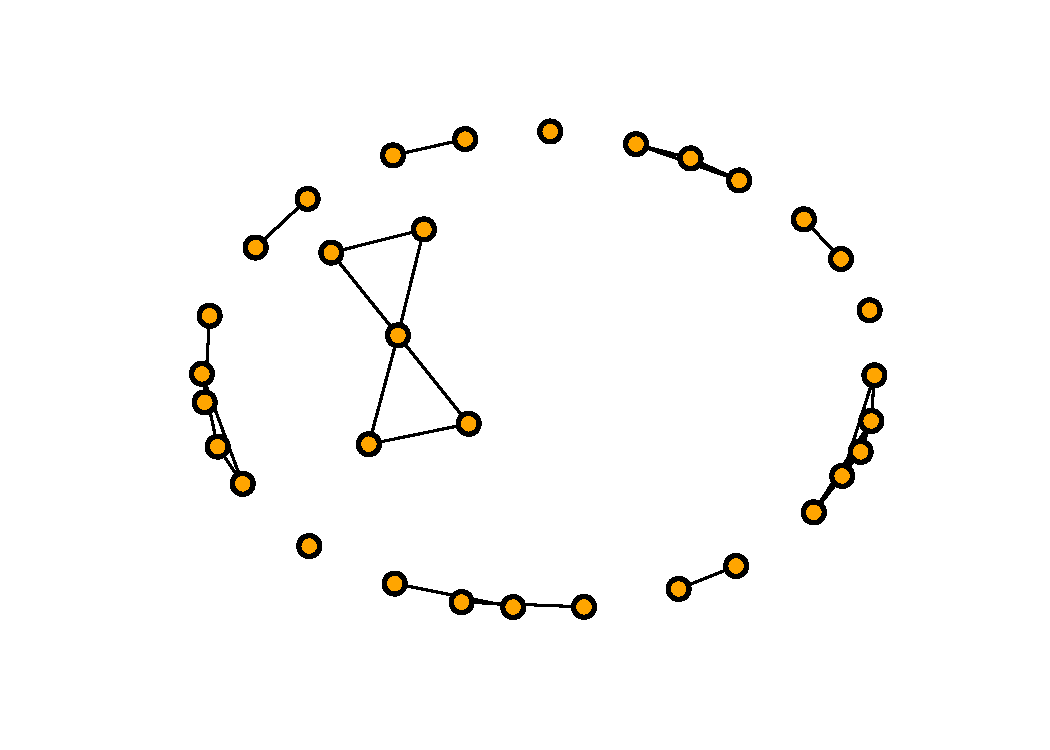
\includegraphics[width=\textwidth]{./assets/images/network_over_period_0.pdf}
            \caption{1961 to 1972}
        \end{subfigure}
        \begin{subfigure}{.22\textwidth}
            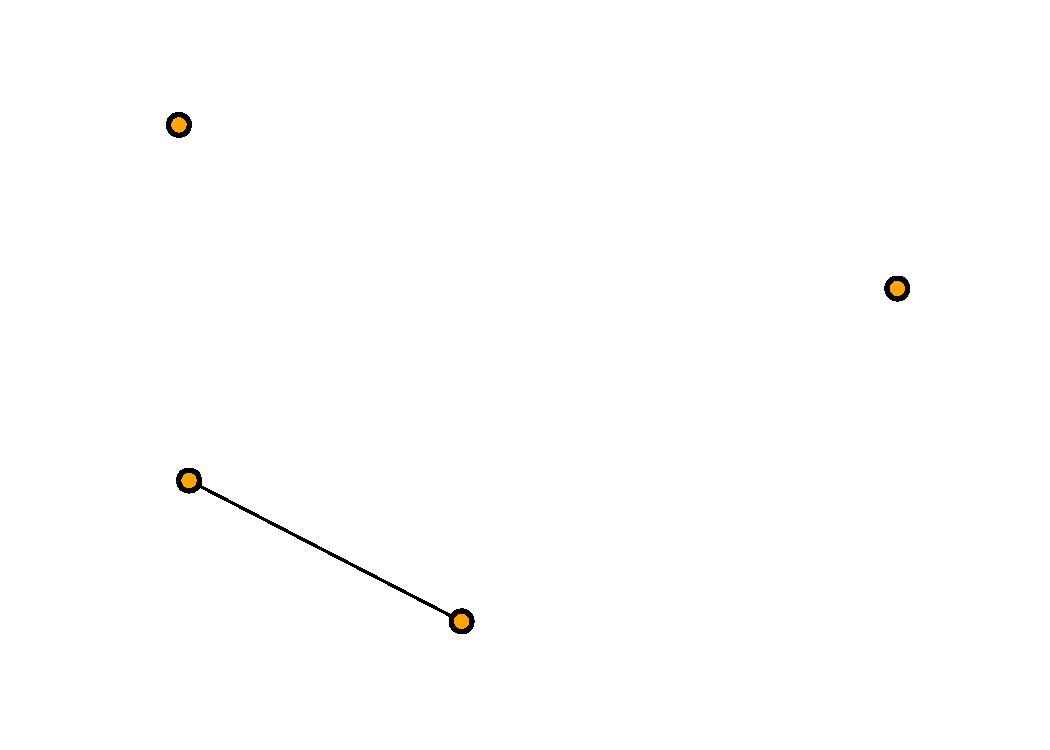
\includegraphics[width=\textwidth]{./assets/images/network_over_period_1.pdf}
            \caption{1981 to 1984}
        \end{subfigure}
        \begin{subfigure}{.22\textwidth}
            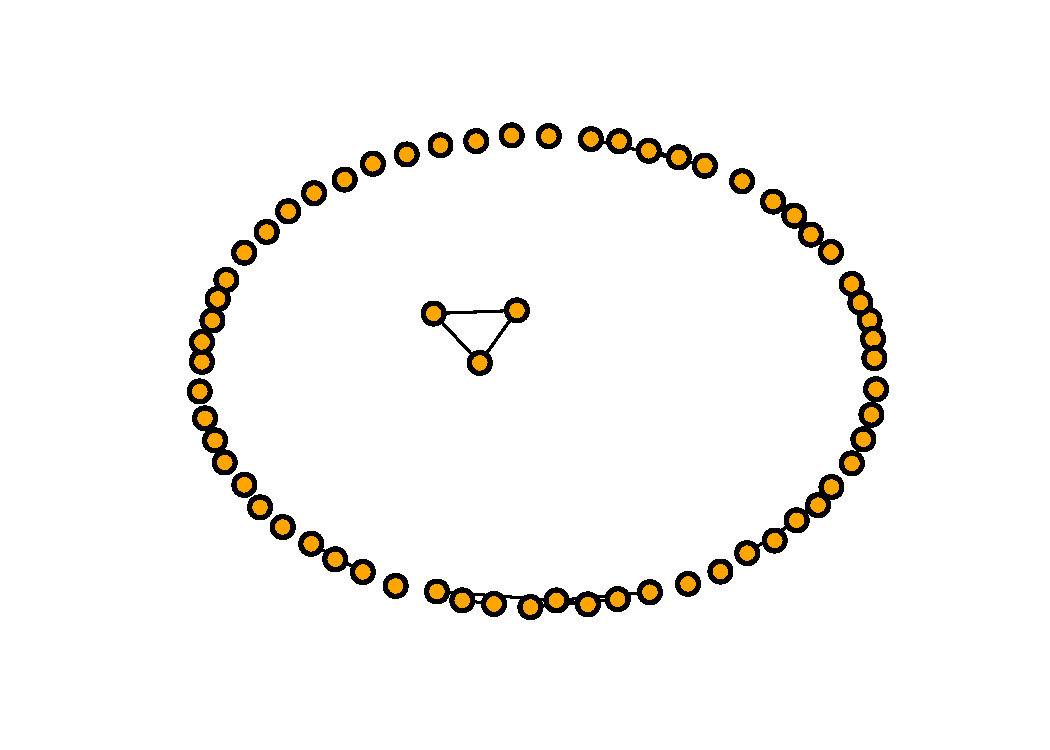
\includegraphics[width=\textwidth]{./assets/images/network_over_period_2.pdf}
            \caption{1984 to 1993}
        \end{subfigure}
        \begin{subfigure}{.22\textwidth}
            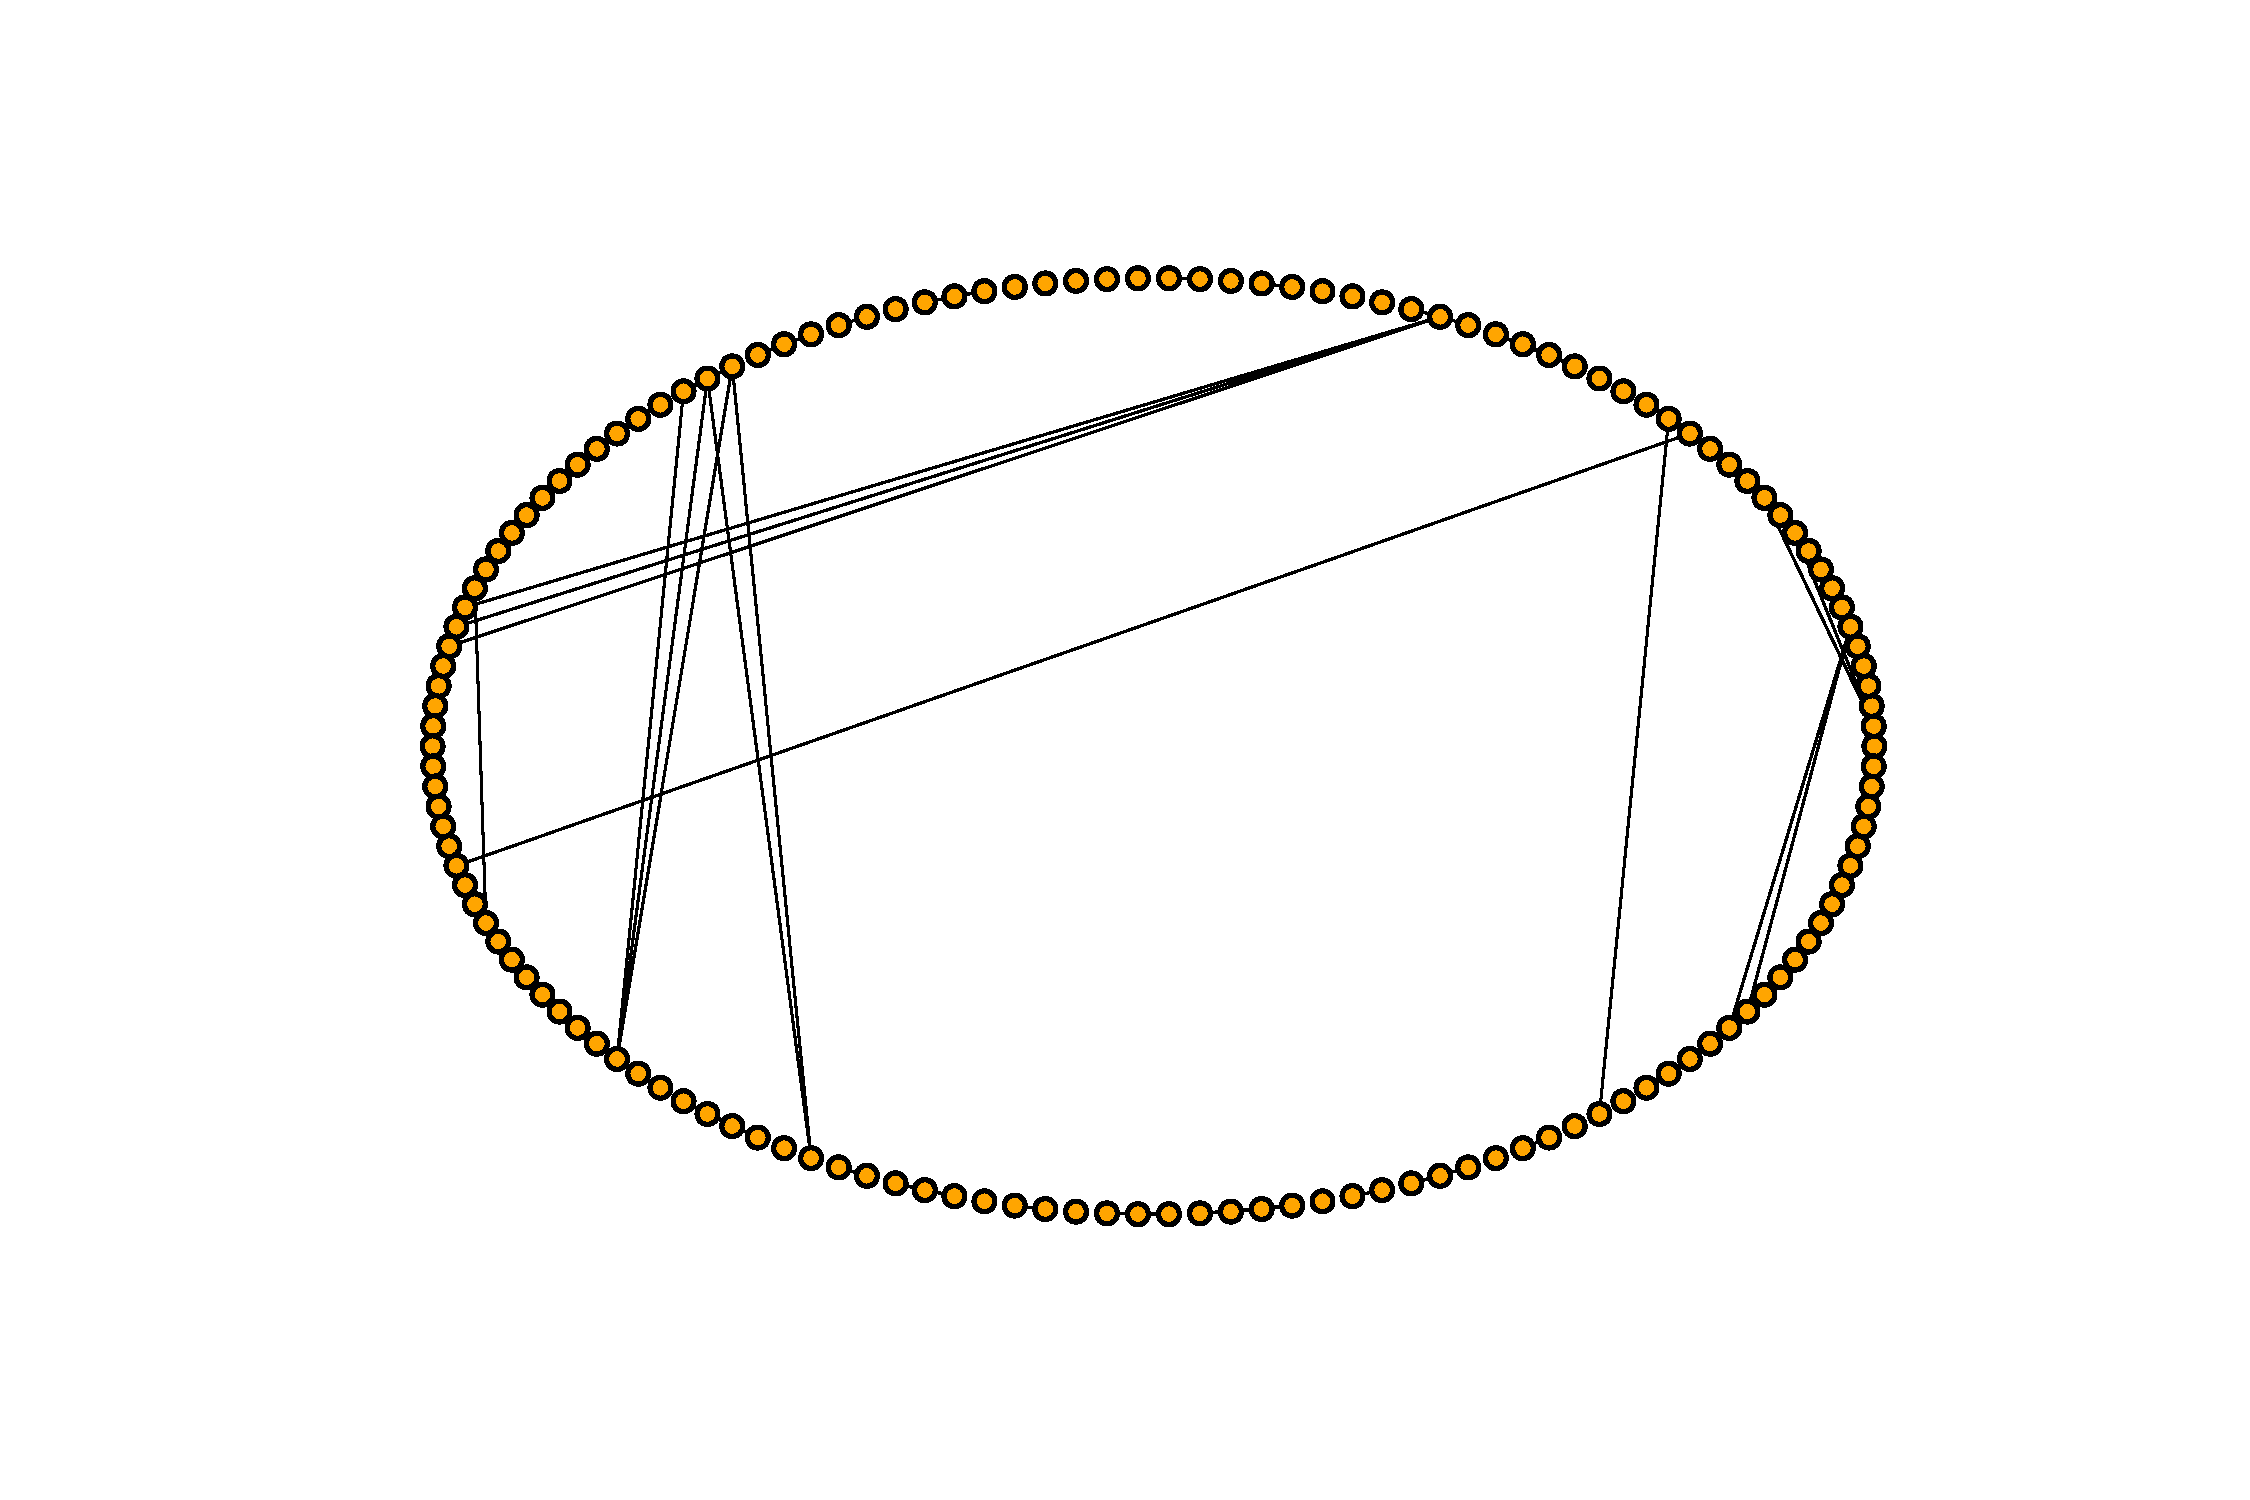
\includegraphics[width=\textwidth]{./assets/images/network_over_period_3.pdf}
            \caption{1987 to 1999}
        \end{subfigure}
        \caption{Co authors networks over time periods.}\label{fig:co_authors_over_time_periods}
    \end{figure} % TODO add legend
    \end{center}

\begin{figure}
    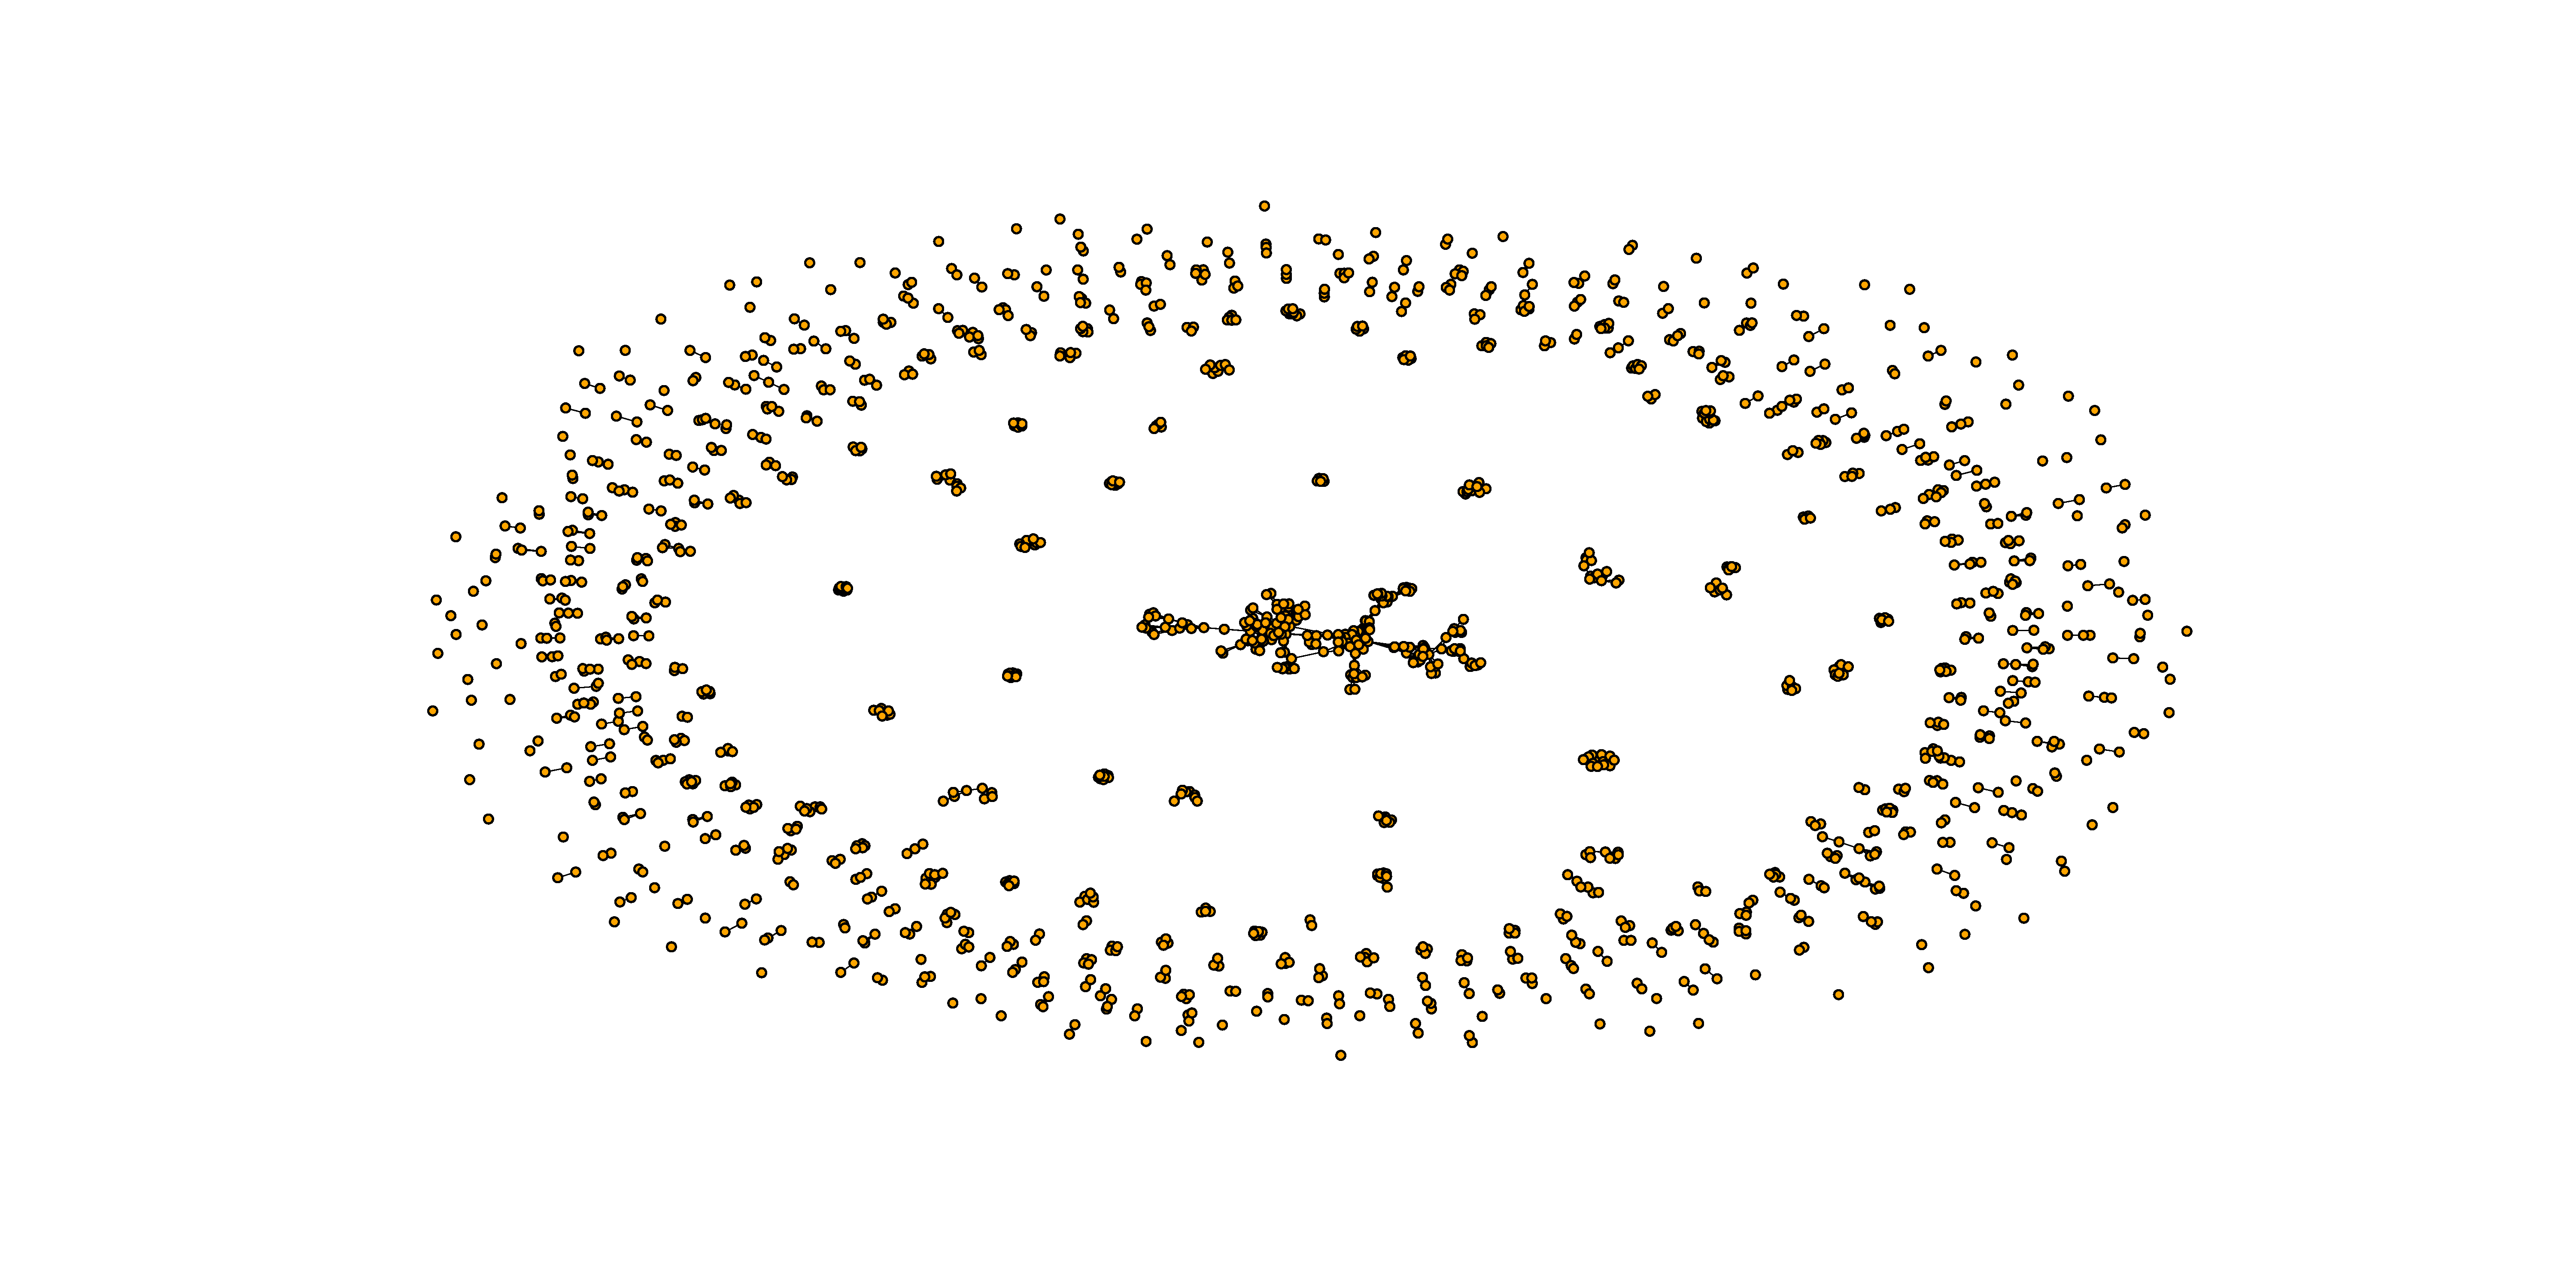
\includegraphics[width=\textwidth]{./assets/images/network_over_period_4.pdf}
    \caption{Co authors network over 1995 to 2015.}\label{fig:co_authors_1995_2015}
\end{figure}

\begin{figure}
    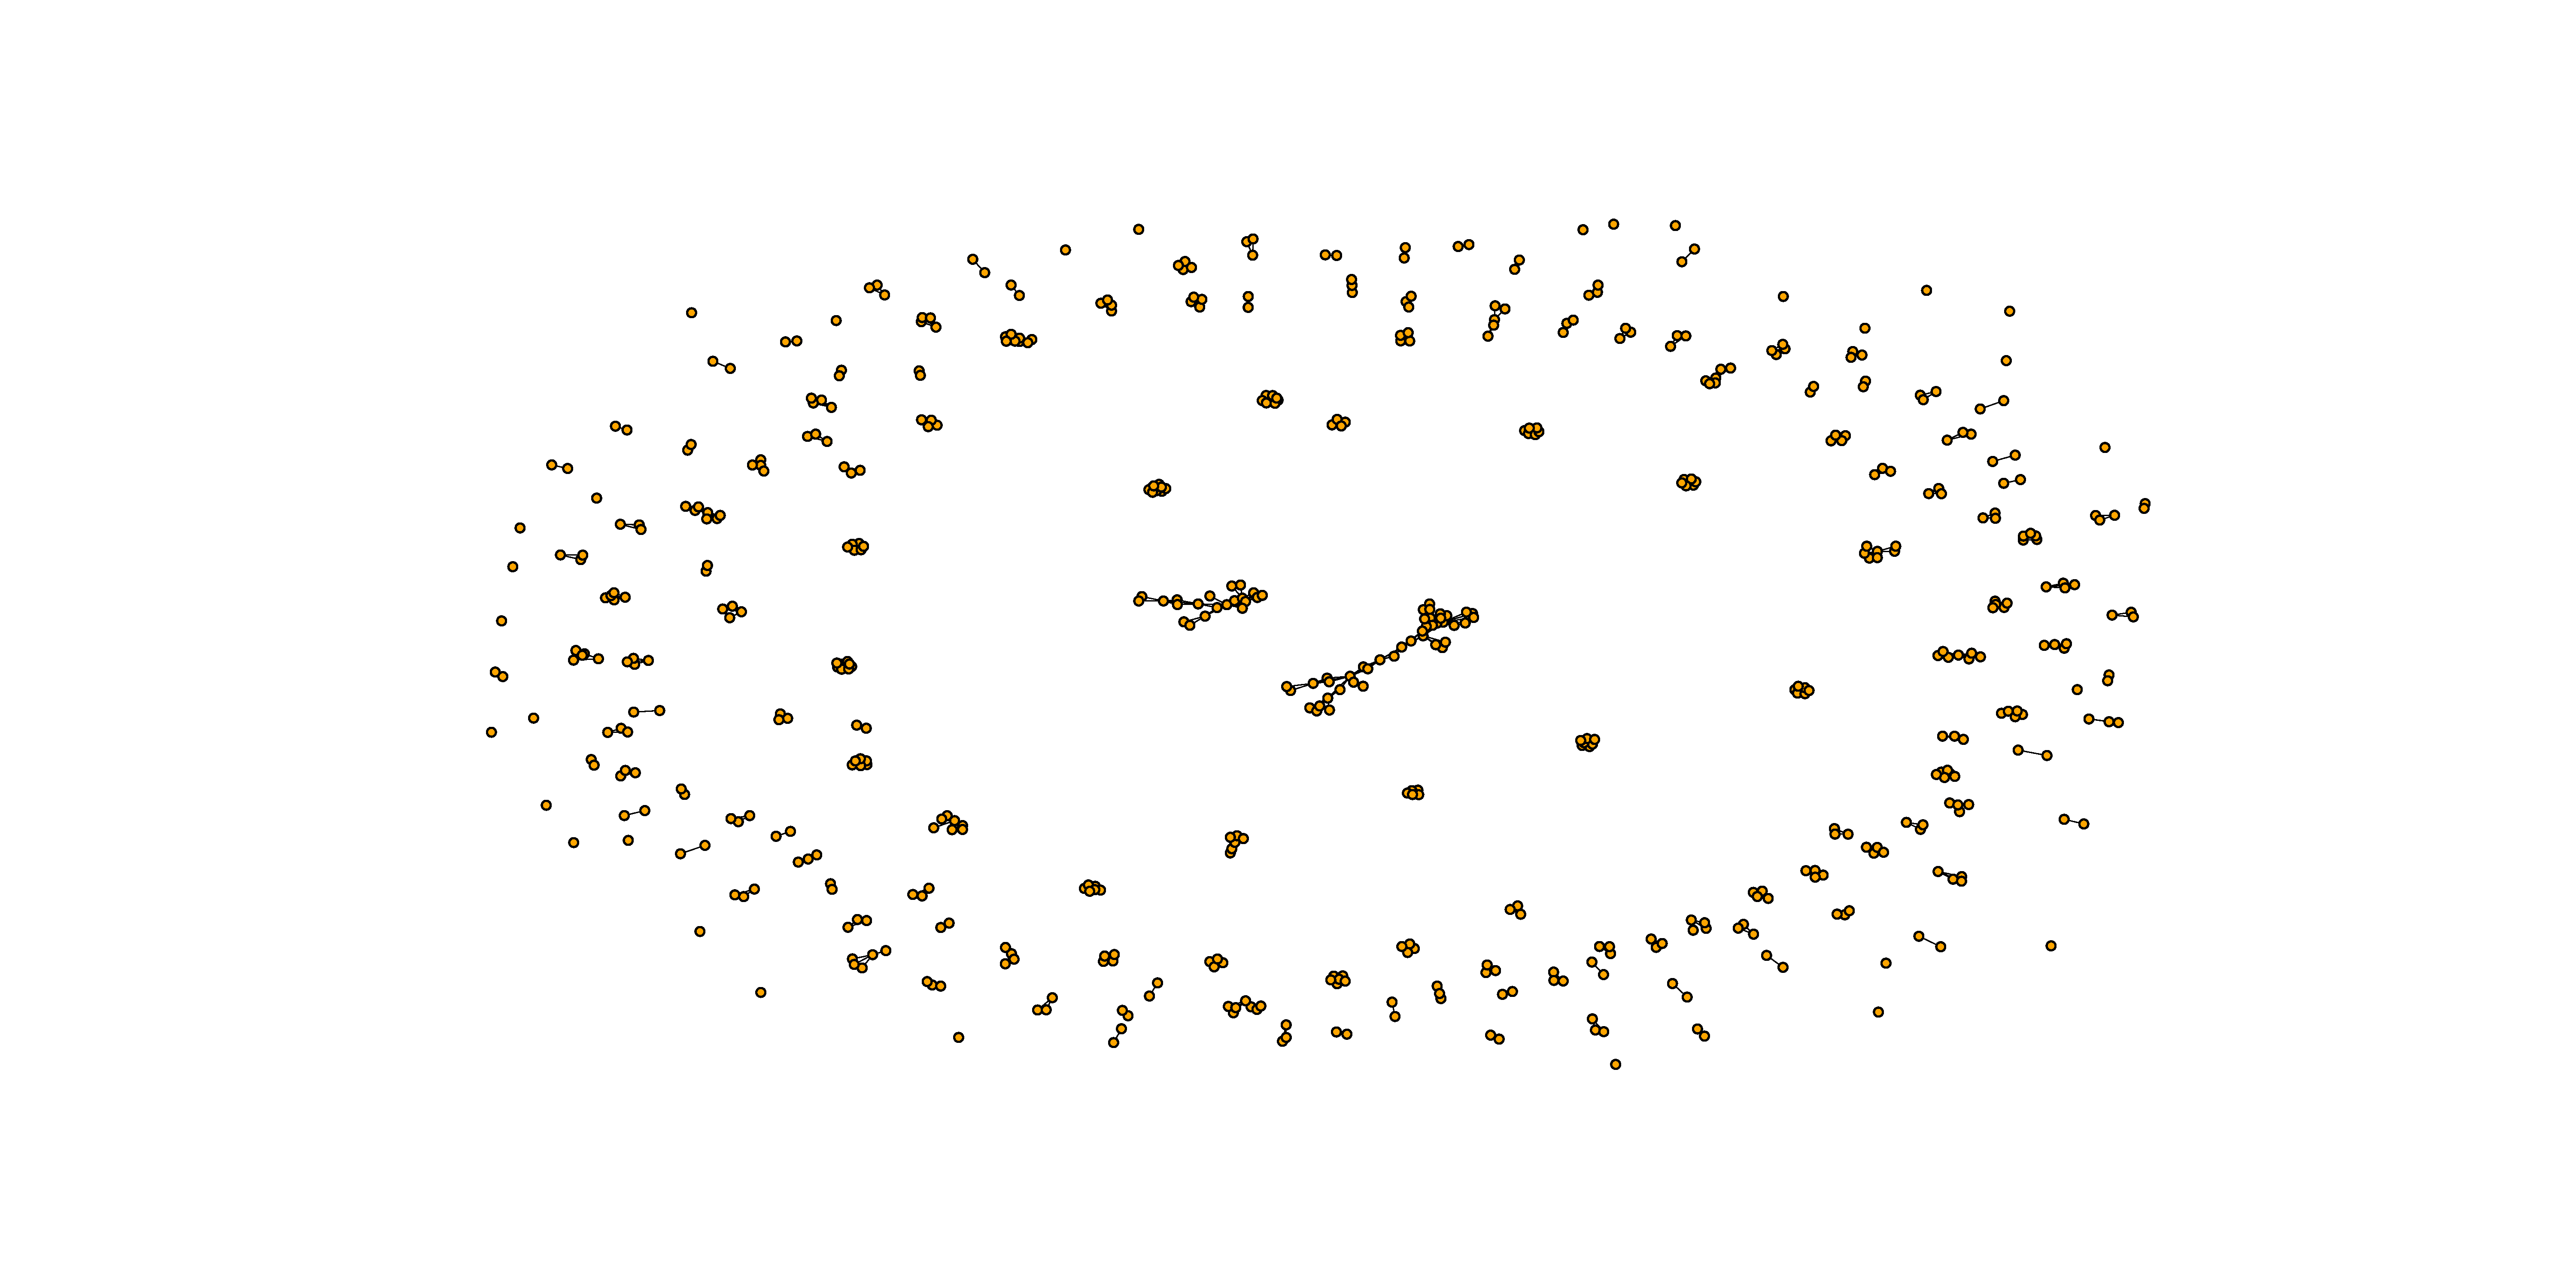
\includegraphics[width=\textwidth]{./assets/images/network_over_period_5.pdf}
    \caption{Co authors network over 2012 to 2015.}\label{fig:co_authors_2012_2015}
\end{figure}

\begin{figure}
    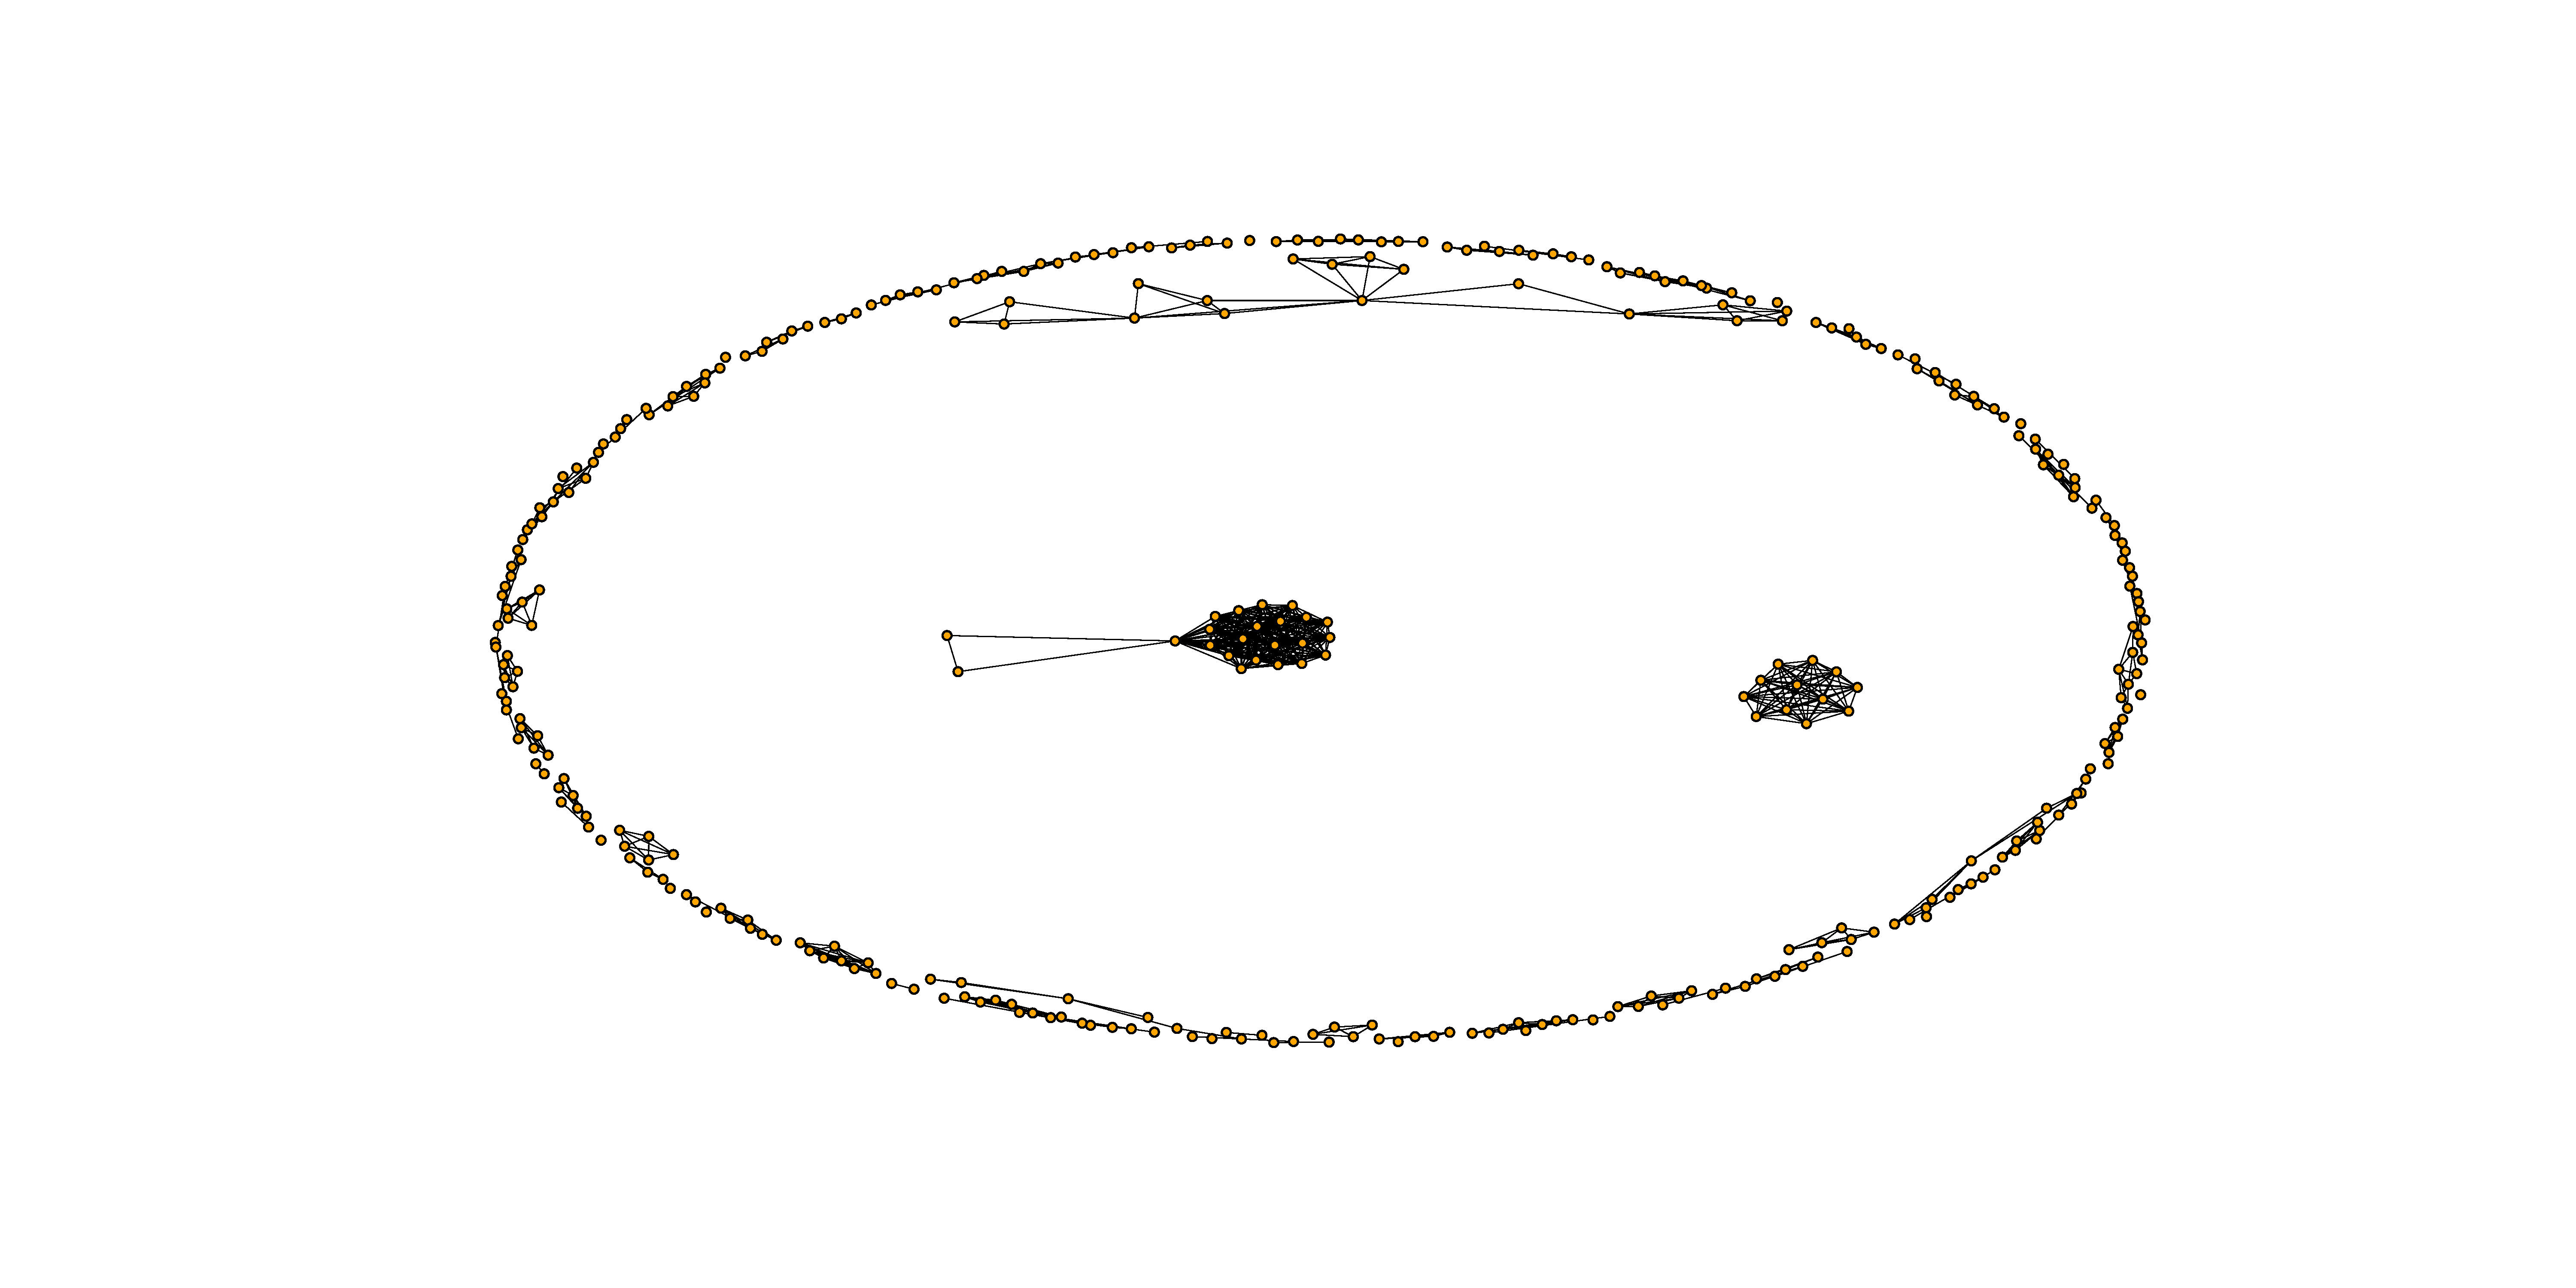
\includegraphics[width=\textwidth]{./assets/images/network_over_period_6.pdf}
    \caption{Co authors network over 2015 to 2017.}\label{fig:co_authors_2015_2017}
\end{figure}

However, what is the number of people that collaborate? Table~\ref{table:size_frequency}
gives the frequency of each size of co authorships. It can be seen that the size
of co-authors varies from 1 to 12 and an outlier of size 21 exists within the data
set as well. The most frequented sizes are those of 3 and 1 authors. Thus within
the field collaboration do exist, but most of them are between 2-3 people.

\begin{table}
    \begin{center}
    \begin{tabular}{lr}
        \toprule
        Size of co authorships &  Frequency \\
        \midrule
        1 & 262 \\
        2 & 139 \\
        3 & 373 \\
        4 & 272 \\
        5 & 26 \\
        6 & 55 \\
        7 & 2 \\
        8 & 4 \\
        9 & 1 \\
        10 & 3 \\
        11 & 4 \\
        12 & 1 \\
        21 & 1 \\
        \bottomrule
    \end{tabular}
    \caption{Co-authors size frequency.}\label{table:size_frequency}
    \end{center}
\end{table}

\subsubsection{Cliques}

The immediate step is to evaluate the co authors cliques. Cliques are 
subsets of vertices, all adjacent to each other, also called complete subgraphs.
Cliques can be looked at is a group of individuals who interact with one another
and have worked on the same projects within the research of the prisoner's dilemma.

A total of 728 cliques exists within the network and the max node number of a
clique is 21. Visualising the subgraphs that exist within the network allow us
to look at the types of collaboration that exist within the field. The following
sub graphs have been generated by looking at cliques with a minimum of 5 vertices
and are not just co-authors of a single paper. 

The first formulation of a clique that was identified is that of Figure
\ref{fig:cliques_0}. Figure \ref{fig:cliques_0} illustrates how
two clusters of several people are connected through a single, or in one case 
two authors. A very common collaborations structure. More interested cases 
arise, shown in Figure~\ref{fig:cliques_1}. These can be viewed as cases
that people worked on the same topic and collaborated with each other but not
all of them thus these are not complete graphs.

\begin{center}
\begin{figure}[!hbtp]
    \begin{subfigure}{0.6\textwidth}
        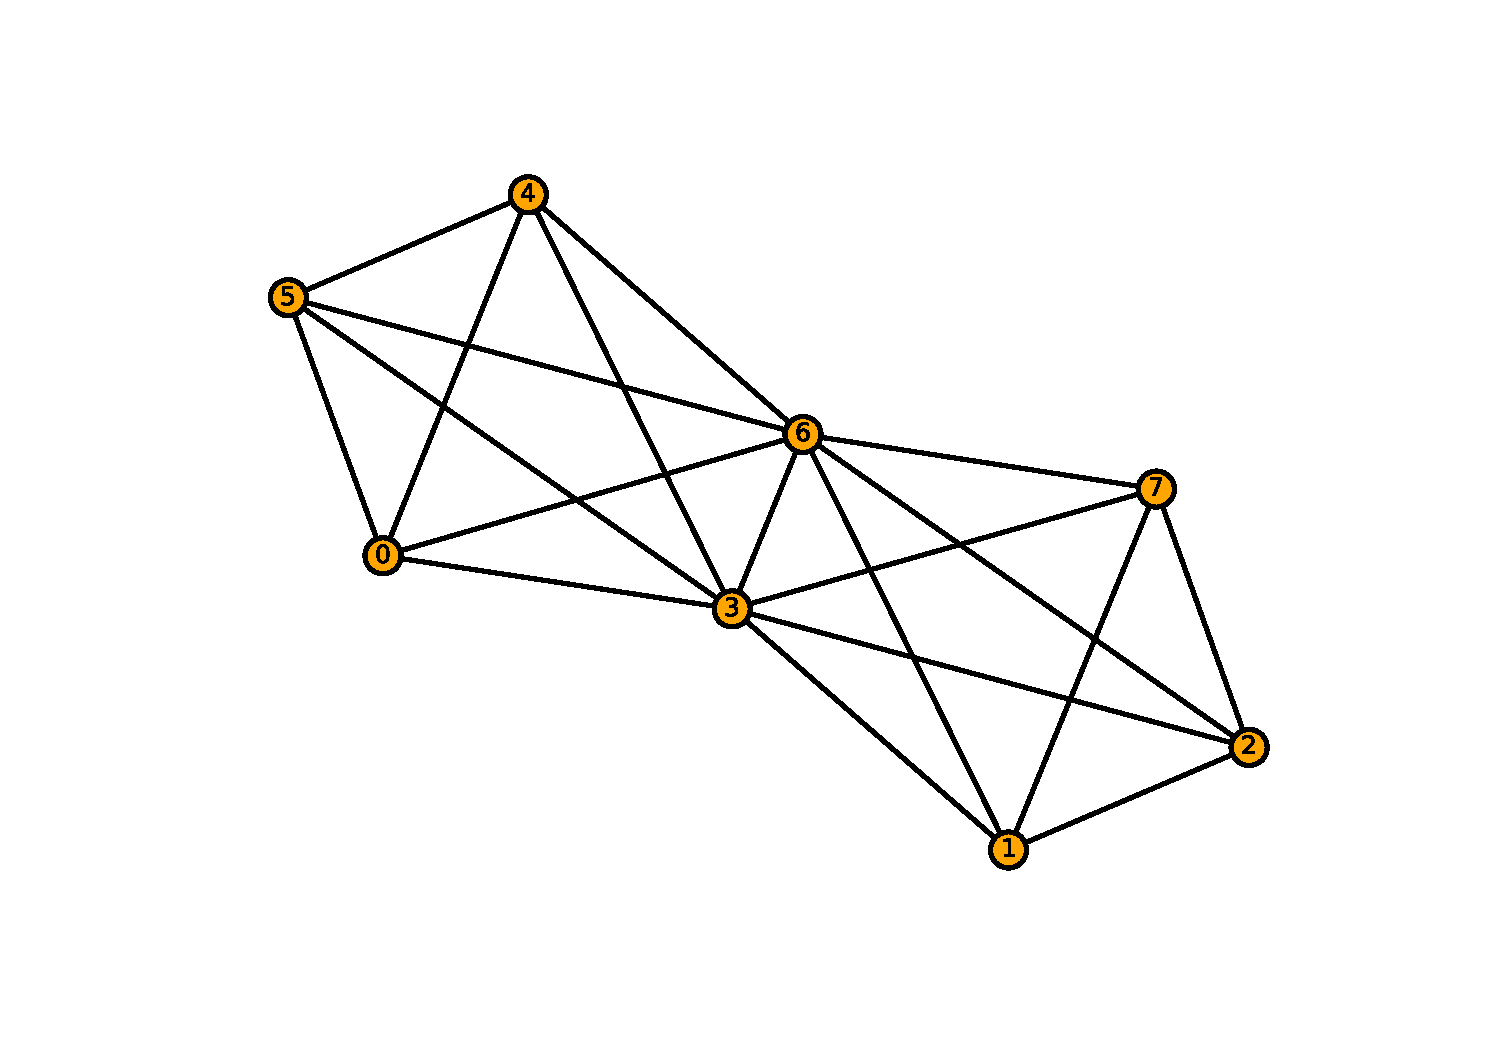
\includegraphics[width=0.6\textwidth]{./assets/images/coauthor00.pdf}
    \end{subfigure}
    \begin{subfigure}{0.6\textwidth}
        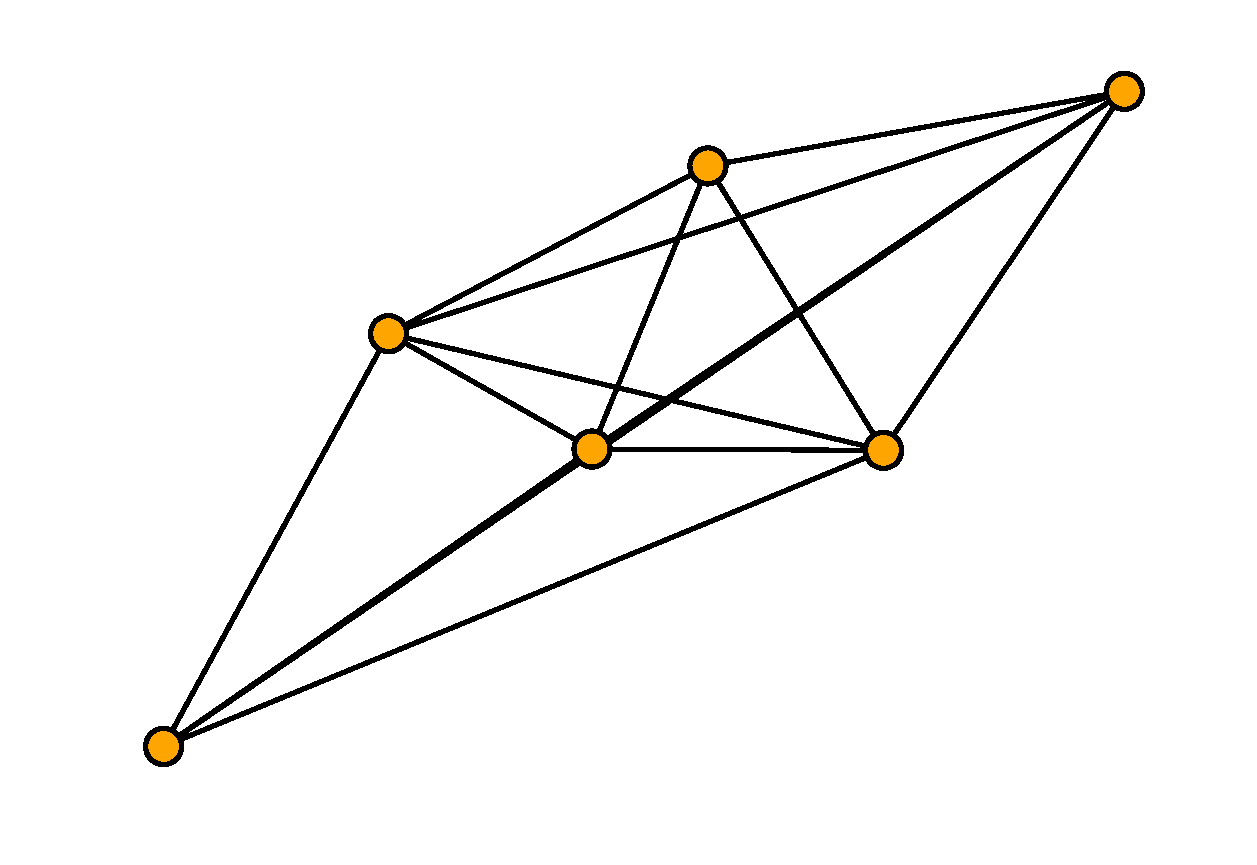
\includegraphics[width=0.6\textwidth]{./assets/images/coauthor04.pdf}
    \end{subfigure}
    \begin{subfigure}{0.6\textwidth}
        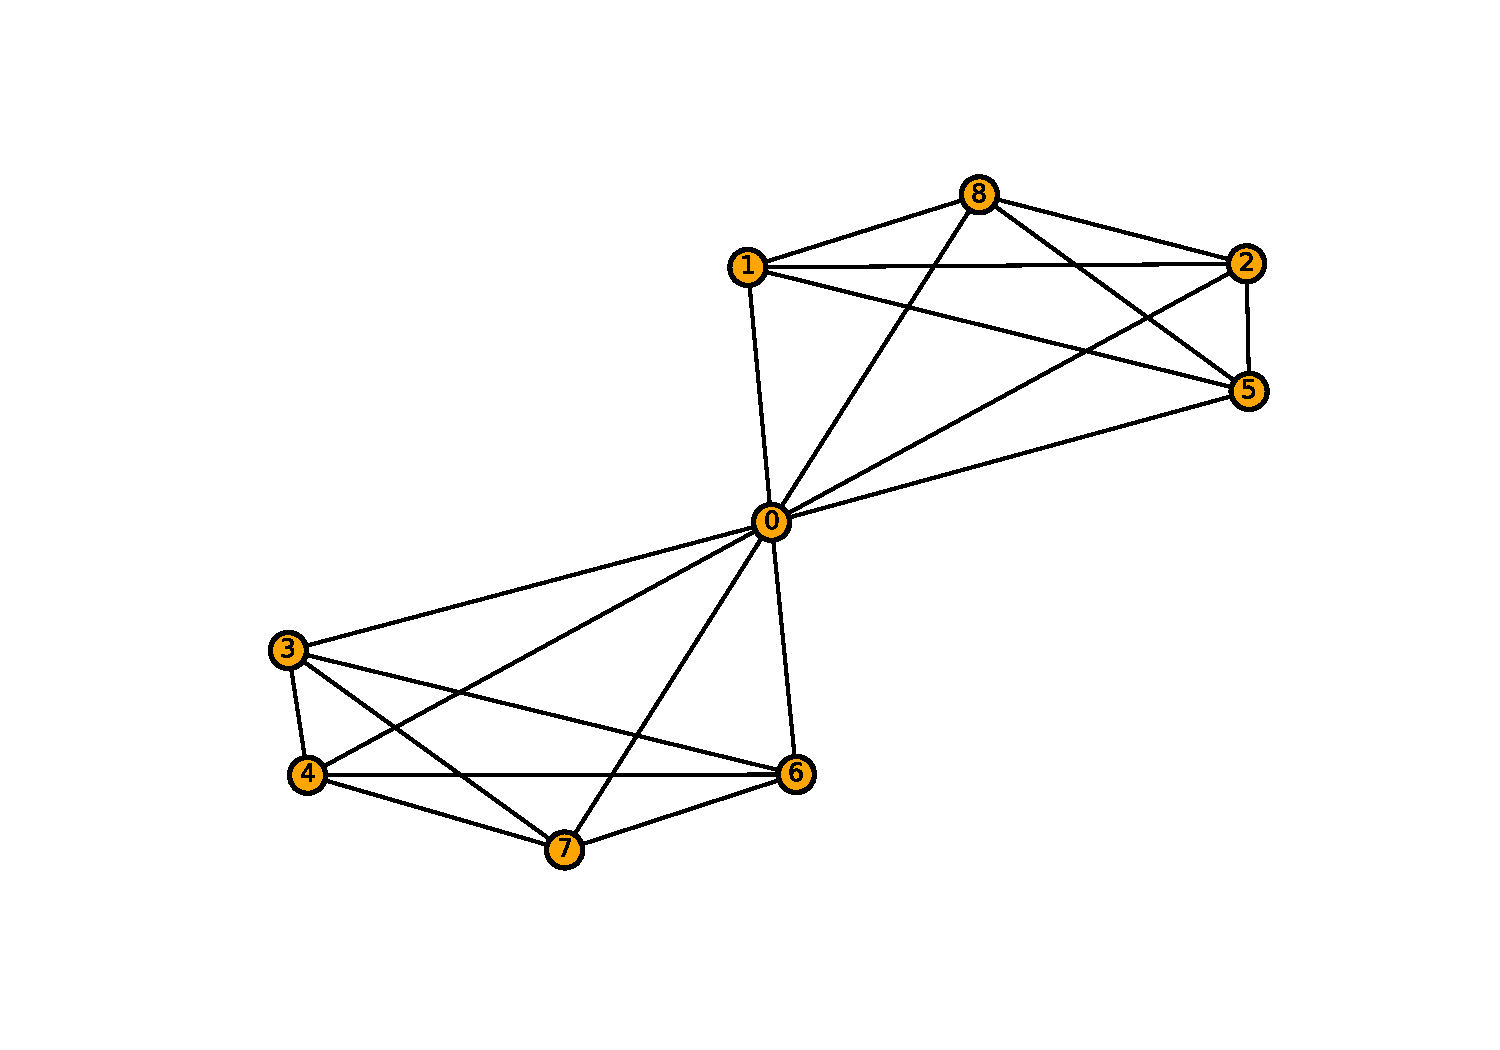
\includegraphics[width=0.6\textwidth]{./assets/images/coauthor06.pdf}
    \end{subfigure}
    \begin{subfigure}{0.6\textwidth}
        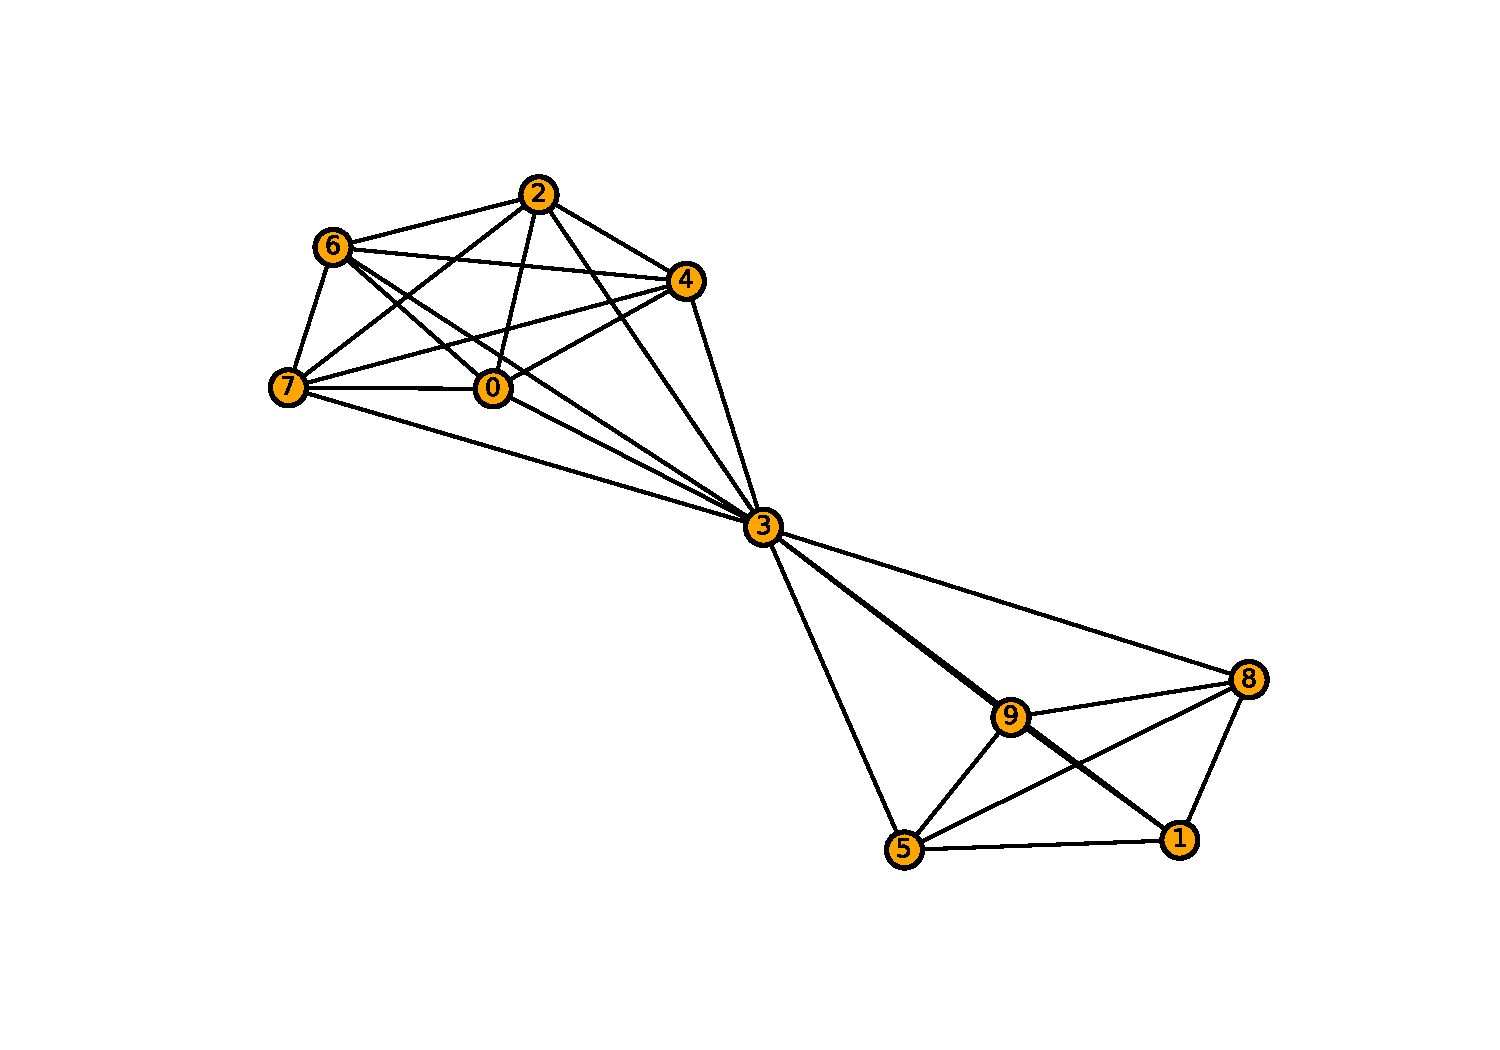
\includegraphics[width=0.6\textwidth]{./assets/images/coauthor07.pdf}
    \end{subfigure}
\caption{Cliques with 1 or 2 central authors.}\label{fig:cliques_0}
\end{figure} % TODO add legend
\end{center}

\begin{figure}[!hbtp]
    \begin{subfigure}{0.35\textwidth}
        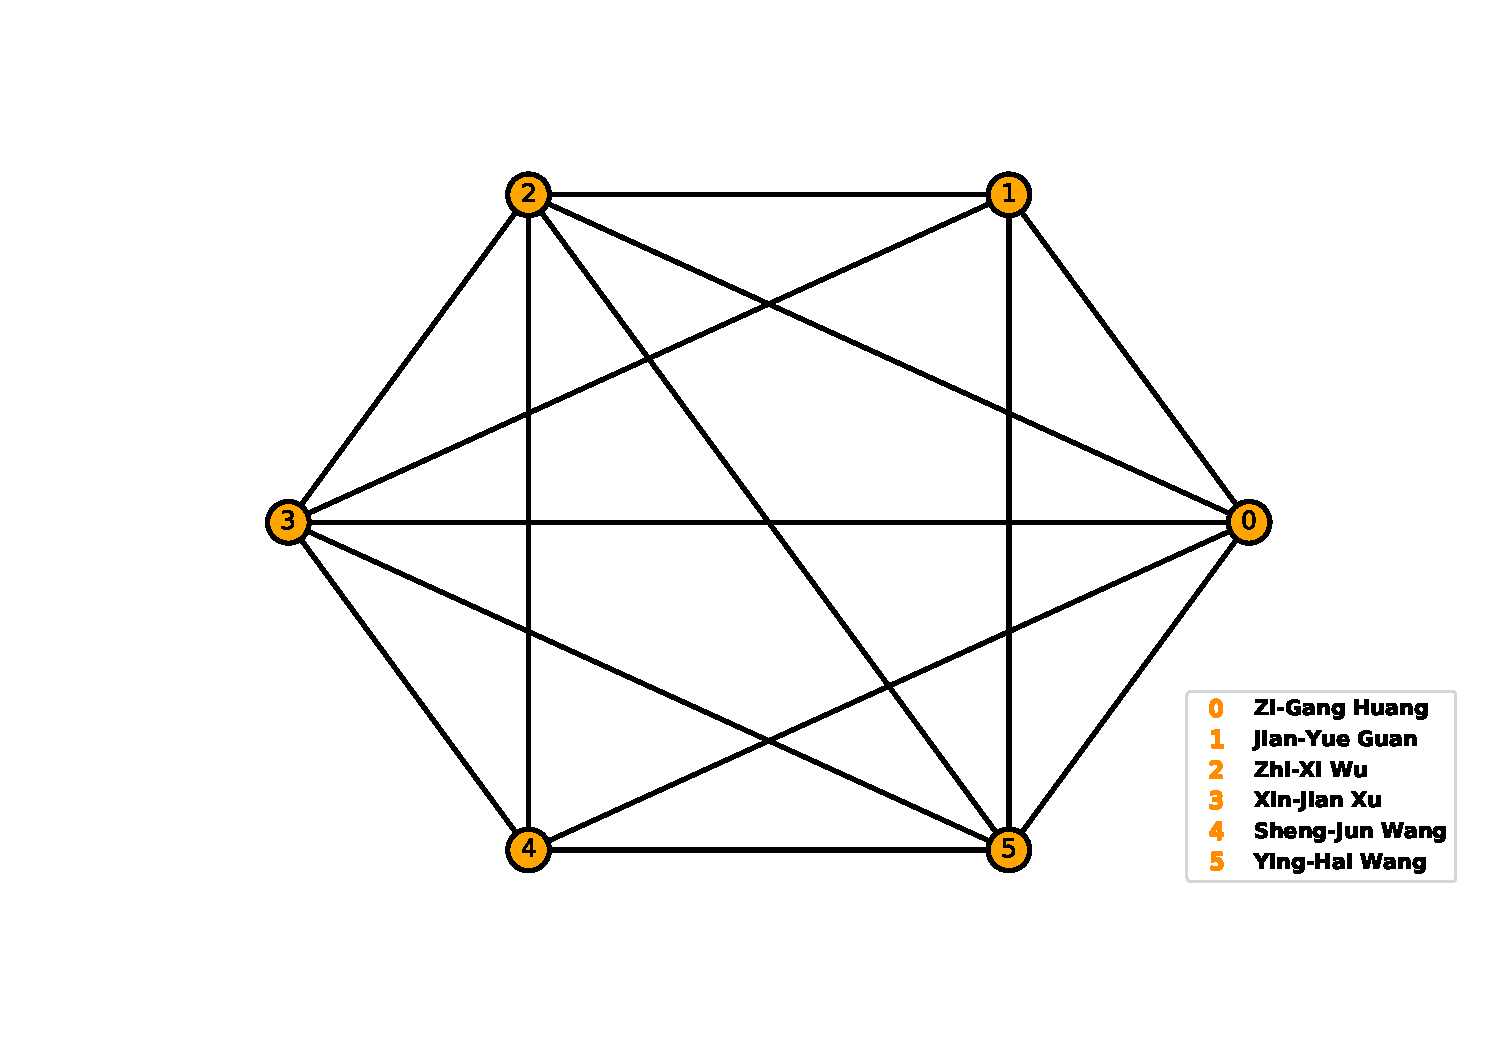
\includegraphics[width=\textwidth]{./assets/images/coauthor01.pdf}
    \end{subfigure}
    \begin{subfigure}{0.35\textwidth}
        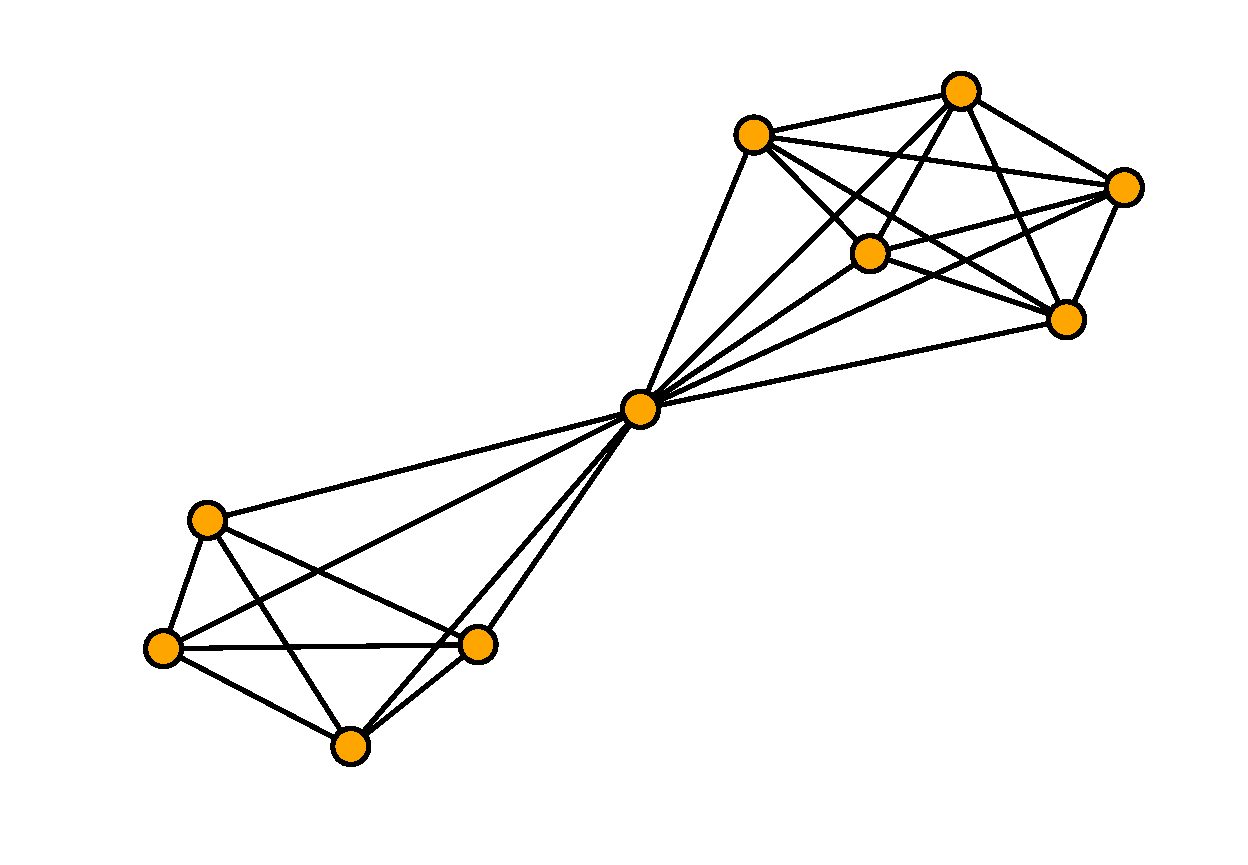
\includegraphics[width=\textwidth]{./assets/images/coauthor02.pdf}
    \end{subfigure}
    \begin{subfigure}{0.35\textwidth}
        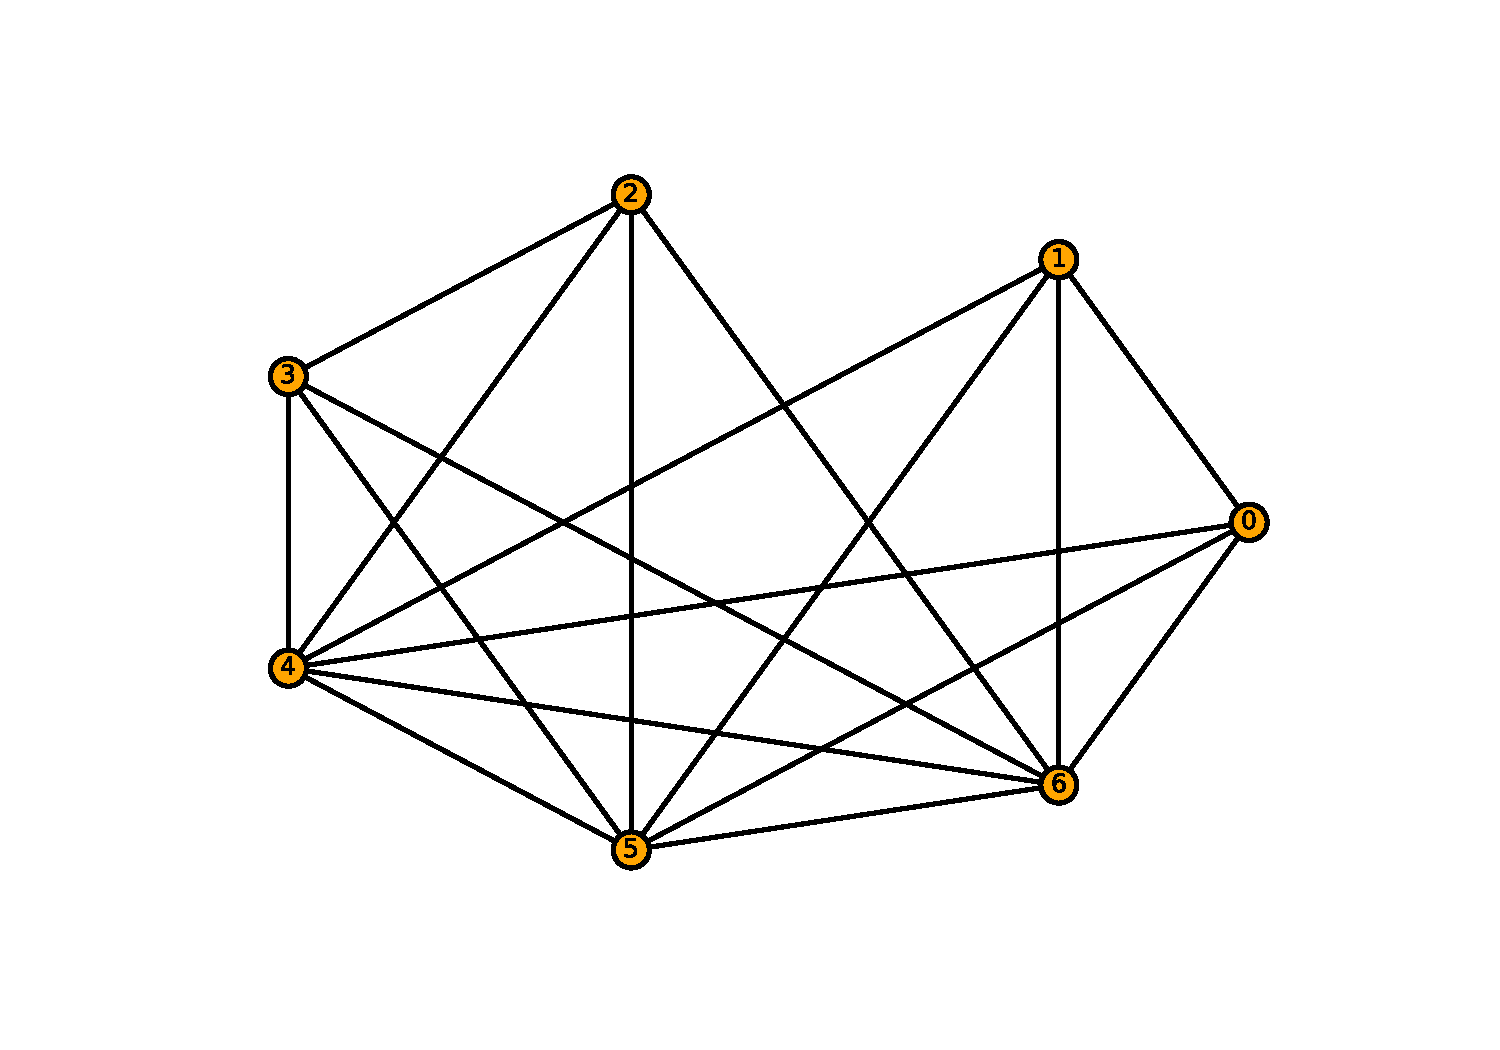
\includegraphics[width=\textwidth]{./assets/images/coauthor03.pdf}
    \end{subfigure}
\caption{Cliques of several connecting authors.}\label{fig:cliques_1}
\end{figure} % TODO add legend

The most interesting cases are those that appear in Figure~\ref{fig:cliques_2}.
The connecting vertices are authors such as.

\begin{figure}[!hbtp]
    \begin{subfigure}{0.5\textwidth}
        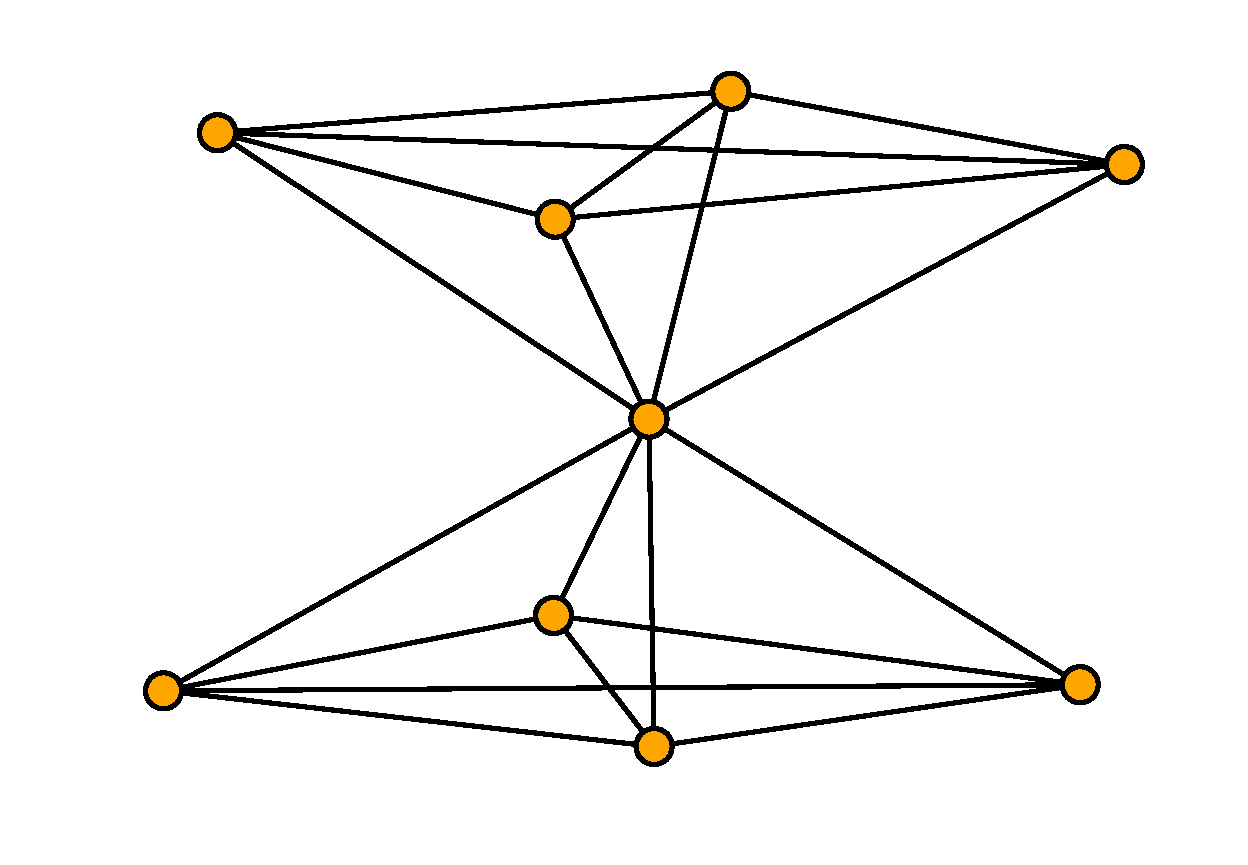
\includegraphics[width=\textwidth]{./assets/images/coauthor05.pdf}
    \end{subfigure}
    \begin{subfigure}{0.5\textwidth}
        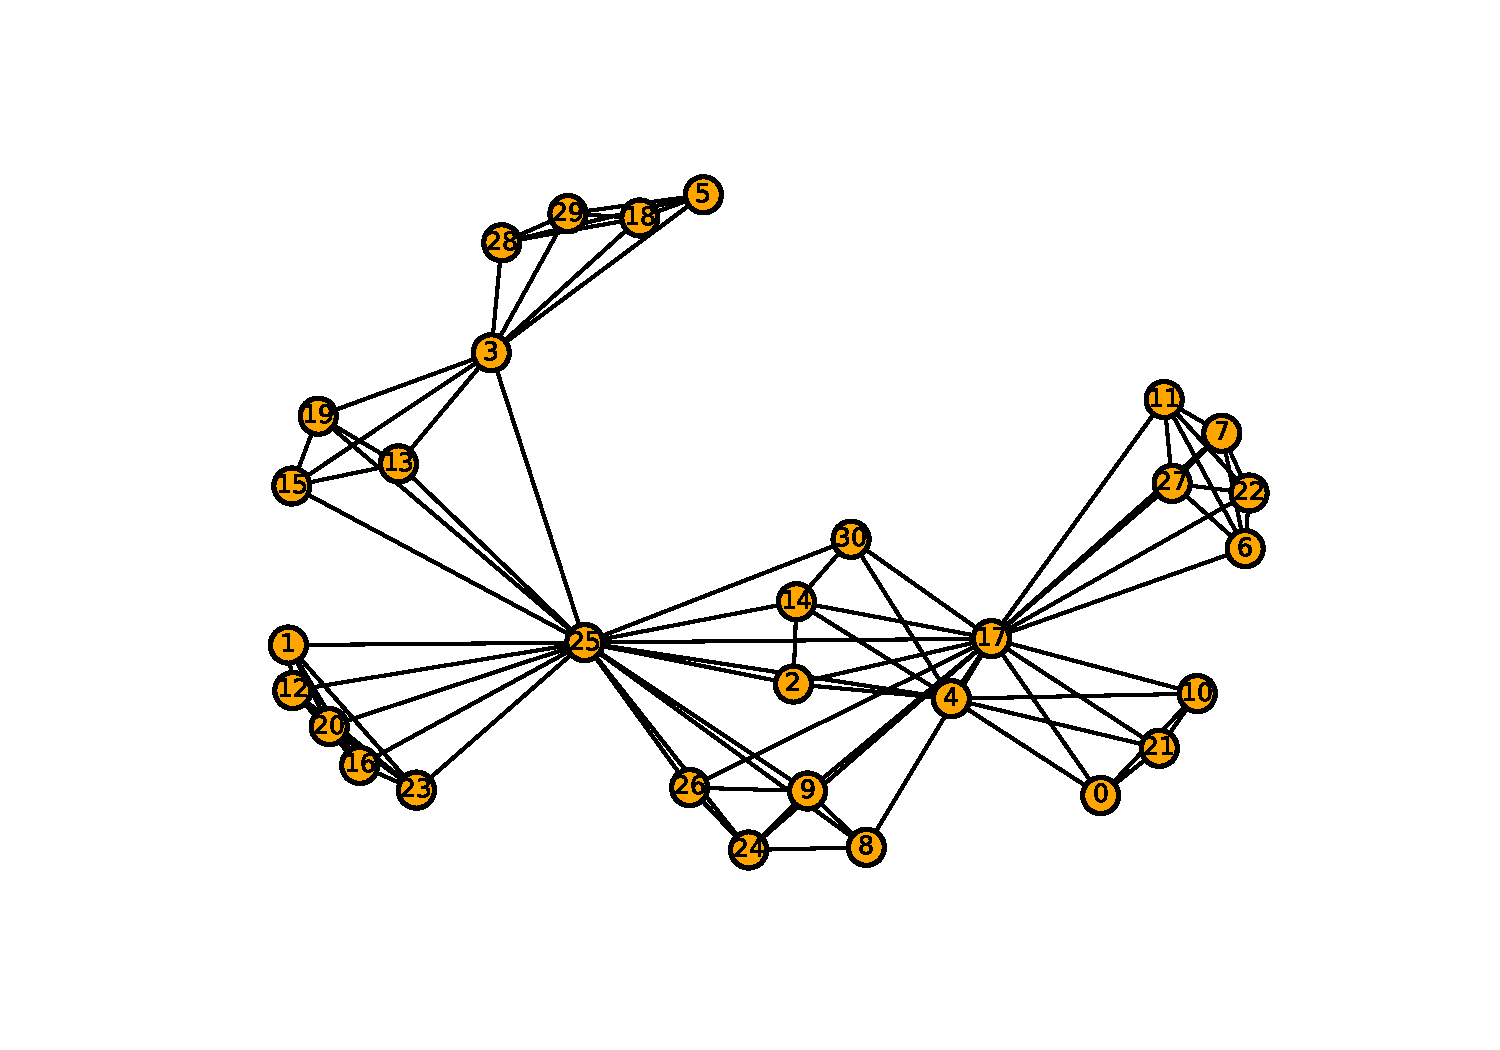
\includegraphics[width=\textwidth]{./assets/images/coauthor08.pdf}
    \end{subfigure}
\caption{Complicated clique networks.}\label{fig:cliques_2}
\end{figure} % TODO add legend


But where are noticeable authors such as Nowak, Ashlock, Plotkin and Axelord? 
Plotkin and Axelrod are authors that have not many collaborations during their
work. On the other hand, Ashlock's and Nowak's cliques are shown below in
Figures.

\bibliographystyle{plain}
\bibliography{bibliography.bib}
\end{document}